\documentclass[10pt,a4paper]{article}
\usepackage[margin=25mm]{geometry}
\usepackage{amsmath,amssymb,amsthm,graphicx,hyperref,bm}
\title{Forward and backward stack operational semantics realize the paired Dialectica procedural interpreter}
\author{Davide Barbarossa, Thomas Powell}
\date{doi:10.4230/LIPIcs.CSL.2026.22; CC BY4.0 (official published text and diagrams)}
\begin{document}
\maketitle
\noindent\textit{Editorial note.} Copyright Davide Barbarossa and Thomas Powell; official CSL2026.22 CC BY4.0. Count one paired operational adequacy result under exact while descent assumptions. Supporting rules, soundness theorems, examples and individual directions are not additional targets.\par\medskip
\noindent\textit{Allowed standard prerequisites (editorial).}\begin{itemize}
\item Higher-order Heyting arithmetic WE-HA omega, SystemT and standard wellfounded induction/finite-sequence representation. Original Section2 and references18/19 plus exact current abstract-type/while extension. Finite sequences are stated by the authors to be encodable but encoding details omitted; no encoding proof is generated. All current backward-while constructors and operational adequacy proof are actually retained.
\end{itemize}\medskip

% BEGIN S2
 
\par\medskip\noindent\textbf{2 Preliminaries}\par
 
% BEGIN S2.SS0.SSS0.Px1
 
\par\medskip\noindent\textbf{The base system $\mathrm{WE}\mbox{-}\mathrm{HA}^{\omega}$}\par
 
% BEGIN S2.SS0.SSS0.Px1.p1
 
Essentially all applications of Dialectica to concrete proofs in mathematics can be described formally in terms of some theory based on arithmetic in all finite types, and accordingly we take as our base theory the weakly extensional version $\mathrm{WE}\mbox{-}\mathrm{HA}^{\omega}$ of higher-order Heyting arithmetic, the higher-order theory of intuitionistic arithmetic with all finite types, whose underlying programming language of terms corresponds to System T. This can be simultaneously used as a system for formalising mathematics, or as a logic for reasoning about higher-order programs, and we take both perspectives in this paper. Full details can be found in [18, Chapter 3], and the very brief overview here is merely used as an opportunity to fix notational conventions. The types of $\mathrm{WE}\mbox{-}\mathrm{HA}^{\omega}$ are the simple types\par
  
\par  \quad  \[X,Y::=\mathsf{nat}\,|\,X\to Y\]\quad  \quad  
  
where $\mathsf{nat}$ represents a base type of natural numbers. As in conventional in proof mining, we work with sequences of types in the metalanguage rather than explicitly introducing product types, which in particular allows us to employ more liberal abbreviations in the logical system. We use boldface $\bm{X}=X_{1},\ldots,X_{n}$ to denote sequences of types, and from now on, when we say “type” we usually refer to a sequence. Similarly, we use boldface $\bm{a}=a_{1},\ldots,a_{n}$ to denote sequences of terms, writing $\bm{a}:\bm{X}$ or $\bm{a}^{\bm{X}}$ to denote $a_{1}:X_{1},\ldots,a_{n}:X_{n}$.\par
 
% END S2.SS0.SSS0.Px1.p1
 
% BEGIN S2.SS0.SSS0.Px1.p2
 
The terms of $\mathrm{WE}\mbox{-}\mathrm{HA}^{\omega}$ are those of the simply typed $\lambda$-calculus plus constants $\mathsf{0}:\mathsf{nat}$ and $\mathsf{suc}:\mathsf{nat}\to\mathsf{nat}$ for zero and successor (we use $x+1$ for $\mathsf{suc}\,x$) and, for each sequence $\bm{X}$ of types, a constant $\bm{\mathtt{rec}}_{\bm{X}}:(\mathsf{nat}\to\bm{X}\to\bm{X})\to\bm{X}\to\mathsf{nat}\to\bm{X}$ for primitive recursion. We include an explicit cases constructor $\mathtt{if}({b^{\mathsf{nat}}},{\bm{s}},{\bm{t}})$ for all types, even though this is definable from the recursor. We make free use of a number of standard abbreviations around sequences of types and terms. If $\bm{X}=X_{1},\ldots,X_{n}$ and $\bm{Y}=Y_{1},\ldots,Y_{m}$ then $\bm{X}\to\bm{Y}$ denotes the sequence $(X_{1}\to\ldots\to X_{n}\to Y_{j})^{m}_{j=1}$, Similarly, if $\bm{a}:\bm{X}\to\bm{Y}$ and $\bm{b}:\bm{X}$, then by $\bm{a}\bm{b}:\bm{Y}$ we mean $(a_{j}b_{1}\ldots b_{n})^{m}_{j=1}$, and if $\bm{c}:\bm{Y}$ are terms and $\bm{x}:\bm{X}$ are variables, then by $\lambda\bm{x}.\bm{c}:\bm{X}\to\bm{Y}$ we mean$(\lambda x_{1},\ldots,x_{n}.c_{j})^{m}_{j=1}$. We write $\bm{b},\bm{c}:\bm{X},\bm{Y}$ for the concatenation of two sequences.\par
 
% END S2.SS0.SSS0.Px1.p2
 
% BEGIN S2.SS0.SSS0.Px1.p3
 
Formulas of $\mathrm{WE}\mbox{-}\mathrm{HA}^{\omega}$ are built from atomic formulas of the form $t=_{\mathsf{nat}}s$ for $t,s:\mathsf{nat}$, the usual logical connectives $\vee,\wedge,\to,\top,\bot$ (where we write $\neg A:=A\to\bot$), and quantifiers $\forall^{X},\exists^{X}$ for each simple type $X$ (which we usually omit). We also write $\exists\bm{x}\,A(\bm{x})$ for $\exists^{X_{1}}x_{1},\ldots,\exists^{X_{n}}x_{n}\,A(x_{1},\ldots,x_{n})$ and similarly for $\forall$. Equality $=_{X}$ at higher types is defined in terms of $=_{\mathsf{nat}}$, where for $X=X_{1}\to\ldots\to X_{n}\to\mathsf{nat}$ we set\par
  
\par  \quad  \[t=_{X}s:=\forall x_{1},\ldots,x_{n}(tx_{1}\ldots x_{n}=_{\mathsf{nat}}sx_{1}\ldots x_{n}).\]\quad  \quad  
  
Equality for sequences is defined in the obvious way. The axioms and rules of $\mathrm{WE}\mbox{-}\mathrm{HA}^{\omega}$ are those of usual intuitionistic logic extended to all simple types, along with equality axioms for $=_{\mathsf{nat}}$, induction, and axioms for the arithmetical constants and terms of System T. For instance, the conditional satisfies\par
  
\par  \quad  \[b=_{\mathsf{nat}}0\to\mathtt{if}({b},{\bm{s}},{\bm{t}})=\bm{s}\ \ \ \mbox{and}\ \ \ b\neq_{\mathsf{nat}}0\to\mathtt{if}({b},{\bm{s}},{\bm{t}})=\bm{t}\]\quad  \quad  
  
and the axioms for the recursors are:\par
  
\par  \quad  \[\mathtt{rec}\,\bm{z}\bm{y}0=\bm{y}\ \ \ \mbox{and}\ \ \ \mathtt{rec}\,\bm{z}\bm{y}(x+1)=\bm{z}x(\mathtt{rec}\,\bm{z}\bm{y}x).\]\quad  \quad  
  
For equality, we consider the weak extensionality rule111We stress that extensionality issues are not a concern for what we do: Soundness theorems for Dialectica are formulated using $\mathrm{WE}\mbox{-}\mathrm{HA}^{\omega}$ for the simple reason that the extensionality axiom is not admissible. However, because our focus in on a descriptive system for realizers, we could equally well work in the fully extensional version of Heyting arithmetic $\mathrm{E}\mbox{-}\mathrm{HA}^{\omega}$.\par
  
\par  \quad  \[\frac{A_{0}\to a=_{X}b}{A_{0}\to B[a/x]\to B[b/x]}\]\quad  \quad  
  
where $B$ is an arbitrary formula and $A_{0}$ is quantifier free. For full details of $\mathrm{WE}\mbox{-}\mathrm{HA}^{\omega}$ the reader is directed to [18], though exact details at this level are unimportant for what follows.\par
 
% END S2.SS0.SSS0.Px1.p3
 
% END S2.SS0.SSS0.Px1
 
% BEGIN S2.SS0.SSS0.Px2
 
\par\medskip\noindent\textbf{The Dialectica interpretation}\par
 
% BEGIN S2.SS0.SSS0.Px2.p1
 
We give a brief overview of the Dialectica interpretation of formulas (as opposed to proofs). This is completely standard, and full details can be found in [18, Chapter 8]. In simple terms, the Dialectica interpretation is a mapping $P\mapsto\exists\bm{x}\forall\bm{y}|{P}|^{\bm{x}}_{\bm{y}}$ that transforms formulas from some source logic (originally Heyting arithmetic) to some higher-order functional language (originally System T). The transformed formula $|{P}|^{\bm{x}}_{\bm{y}}$ contains two additional tuples of free variables, playing the role of witnesses $\bm{x}$ and counterwitnesses $\bm{y}$ for $P$, while the formula $|{P}|^{\bm{x}}_{\bm{y}}$ can be viewed as an orthogonality relation similarly to classical realisability. The aim is to establish that whenever $P$ is provable in the source system, there exists terms $\bm{a}$ such that $\forall\bm{y}|{P}|^{\bm{a}}_{\bm{y}}$ is provable in the target system. For a term $t:\mathsf{nat}$, we introduce a new abbreviation $\vee_{t}$ for the formula\par
  
\par  \quad  \[A\vee_{t}B:=(t=_{\mathsf{nat}}0\to A)\wedge(t\neq_{\mathsf{nat}}0\to B)\]\quad  \quad  
  
Using the fact that any quantifier-free formula $\phi$ of $\mathrm{WE}\mbox{-}\mathrm{HA}^{\omega}$ can be represented by a “characteristic term” $\chi_{\phi}:\mathsf{nat}$ with the same free variables satisfying $\chi_{\phi}=0\leftrightarrow\phi$, we extend this connective to such formulas by defining $A\vee_{\phi}B:=A\vee_{\chi_{\phi}}B$.\par
 
% END S2.SS0.SSS0.Px2.p1
 
% BEGIN Thmtheorem1
 
\par\medskip\noindent\textbf{Definition 1 (Dialectica interpretation [12], see also [18]).}\par
 
% BEGIN Thmtheorem1.p1
 
For a formula $P$ of $\mathrm{WE}\mbox{-}\mathrm{HA}^{\omega}$, we define its Dialectica interpretation to be the formula $\exists\bm{x}\forall\bm{y}\,|{P}|^{\bm{x}}_{\bm{y}}$, whose free variables are the same as $P$, and where $|{P}|^{\bm{x}}_{\bm{y}}$ is a quantifier-free formula, defined inductively along with the types of $\bm{x}$ and $\bm{y}$ as follows:\par
 
% END Thmtheorem1.p1
 
% BEGIN Thmtheorem1.p2
  
\par\noindent  $\blacksquare$ 
% BEGIN S2.I1.i1.p1
 
$|{P}|:=P$ if $P$ is atomic\par
 
% END S2.I1.i1.p1
 
 
\par\noindent  $\blacksquare$ 
% BEGIN S2.I1.i2.p1
 
$|{P\wedge Q}|^{\bm{x},\bm{u}}_{\bm{y},\bm{v}}:=|{P}|^{\bm{x}}_{\bm{y}}\wedge|{Q}|^{\bm{u}}_{\bm{v}}$\par
 
% END S2.I1.i2.p1
 
 
\par\noindent  $\blacksquare$ 
% BEGIN S2.I1.i3.p1
 
$|{P\vee Q}|^{b,\bm{x},\bm{u}}_{\bm{y},\bm{v}}:=|{P}|^{\bm{x}}_{\bm{y}}\vee_{b}|{Q}|^{\bm{u}}_{\bm{v}}$\par
 
% END S2.I1.i3.p1
 
 
\par\noindent  $\blacksquare$ 
% BEGIN S2.I1.i4.p1
 
$|{P\to Q}|^{\bm{f},\bm{F}}_{\bm{x},\bm{v}}:=|{P}|^{\bm{x}}_{\bm{F}\bm{x}\bm{v}}\to|{Q}|^{\bm{f}\bm{x}}_{\bm{v}}$\par
 
% END S2.I1.i4.p1
 
 
\par\noindent  $\blacksquare$ 
% BEGIN S2.I1.i5.p1
 
$|{\exists x\,P(x)}|^{x,\bm{u}}_{\bm{y}}:=|{P(x)}|^{\bm{u}}_{\bm{y}}$\par
 
% END S2.I1.i5.p1
 
 
\par\noindent  $\blacksquare$ 
% BEGIN S2.I1.i6.p1
 
$|{\forall x\,P(x)}|^{\bm{f}}_{x,\bm{y}}:=|{P(x)}|^{\bm{f}x}_{\bm{y}}$\par
 
% END S2.I1.i6.p1
 
  
% END Thmtheorem1.p2
 
% BEGIN Thmtheorem1.p3
 
Note that if $\phi$ is quantifier-free then we can assume that it doesn’t contain $\vee$ (as it can be rewritten as $\chi_{\phi}=0$) and therefore that $|{\phi}|=\phi$.\par
 
% END Thmtheorem1.p3
 
% END Thmtheorem1
 
% BEGIN S2.SS0.SSS0.Px2.p2
 
The characteristic feature of Dialectica, which sets it apart from realisability-like interpretations, is its treatment of implication, which comprises a forward-component $\bm{f}$ as in realisability along with a backward component $\bm{F}$, which together compose in a “backpropagation” style. The soundness theorem for the Dialectica interpretation (i.e. the Dialectica interpretation of proofs), for extensions of $\mathrm{WE}\mbox{-}\mathrm{HA}^{\omega}$, usually takes the following general form:\par
 
% END S2.SS0.SSS0.Px2.p2
 
% BEGIN Thmtheorem2
 
\par\medskip\noindent\textbf{Theorem 2 (Generic soundness theorem).}\par
 
% BEGIN Thmtheorem2.p1
 
Suppose that $\Delta$ is a set of axioms whose Dialectica interpretation is witnessed by terms of $\mathrm{WE}\mbox{-}\mathrm{HA}^{\omega}_{\Delta}$ (provably in this system) for some suitable extension of $\mathrm{WE}\mbox{-}\mathrm{HA}^{\omega}$, and let $\mathcal{U}$ be a set of purely universal formulas. Then whenever\par
  
\par  \quad  \[\mathrm{WE}\mbox{-}\mathrm{HA}^{\omega}+\Delta+\mathcal{U}\vdash P\]\quad  \quad  
  
we can extract terms $\bm{a}$, whose free variables are the same as those of $P$, such that\par
  
\par  \quad  \[\mathrm{WE}\mbox{-}\mathrm{HA}^{\omega}_{\Delta}+\mathcal{U}\vdash\forall\bm{y}|{P}|^{\bm{a}}_{\bm{y}}.\]\quad  \quad  
  
% END Thmtheorem2.p1
 
% END Thmtheorem2
 
% BEGIN S2.SS0.SSS0.Px2.p3
 
In particular, we can set $\Delta=\mathcal{U}=\emptyset$ to obtain the Dialectica interpretation of $\mathrm{WE}\mbox{-}\mathrm{HA}^{\omega}$. A common formulation (cf. [18, Theorem 8.6]) has $\Delta$ consisting of the axiom of choice ($\mathrm{AC}$), the independence of premise scheme for universal formulas ($\mathrm{IP}^{\omega}_{\forall}$), and Markov’s principle ($\mathrm{M}^{\omega}$) with $\mathrm{WE}\mbox{-}\mathrm{HA}^{\omega}_{\Delta}=\mathrm{WE}\mbox{-}\mathrm{HA}^{\omega}$. A further extension is to add the double negation shift to $\Delta$, and then $\mathrm{WE}\mbox{-}\mathrm{HA}^{\omega}_{\Delta}=\mathrm{WE}\mbox{-}\mathrm{HA}^{\omega}+(\mathrm{BR})$ i.e. Heyting arithmetic extended with bar recursion in all finite types (cf. [18, Chapter 11]).\par
 
% END S2.SS0.SSS0.Px2.p3
 
% END S2.SS0.SSS0.Px2
 
% END S2


% BEGIN S3
 
\par\medskip\noindent\textbf{3 The action of Dialectica on programs}\par
 
% BEGIN S3.p1
 
We now present the soundness theorem for the Dialectica interpretation from a slightly different perspective, by providing a collection of specification rules for Dialectica realizers (terminology we use for programs extracted from proofs using Dialectica), all of which are sound in our base theory $\mathrm{WE}\mbox{-}\mathrm{HA}^{\omega}$. The intention here is to construct a rich, descriptive language where the focus is on the realizing terms rather than the underlying logic, one which can be easily extended with new programming constructs, or new rules for describing extracted programs of a specific type. We give several examples of this in what follows.\par
 
% END S3.p1
 
% BEGIN S3.p2
 
Our basic approach is inspired by Hoare logic [14], in the sense that our rules apply to “triples” that describe properties of Dialectica realizers. Let us explain this in more detail. Viewed abstractly, a basic Hoare triple $\{P\}\,{c}\,\{Q\}$ describes the effect of some command $c$ in an imperative language on an underlying state. Here $P$ (the precondition) and $Q$ (the postcondition) are assertions about the state, and the meaning of the triple is that whenever the command executes on a state satisfying $P$, the resulting state satisfies $Q$. We can represent this basic idea in predicate logic by viewing the pre- and postconditions as formulas $P(s),Q(s)$ acting on objects $s:S$ for some state type $S$, and commands as functions $c:S\to S$. The Hoare triple then becomes the statement that $c$ satisfies\par
  
\par  \quad  \[\forall s(P(s)\to Q(cs)).\]\quad  \quad  
  
If we now imagine that $P(s)$ and $Q(s)$ are quantifier-free formulas, and the state can be encoded in a suitable way in $\mathrm{WE}\mbox{-}\mathrm{HA}^{\omega}$, the formula $P(s)\to Q(cs)$ is exactly\par
  
\par  \quad  \[|{\exists x\,P(x)\to\exists x\,Q(x)}|^{c}.\]\quad  \quad  
  
With this loose correspondence in mind, we now generalise to formulas of arbitrary logical complexity and define a “Dialectica triple” as\par
  
\par  \quad  \[{P}\,{\langle{\bm{a}}\,|\,{\bm{\alpha}}\rangle}\,{Q}:=\forall\bm{x},\bm{v}\,|{P\to Q}|^{\bm{a},\bm{\alpha}}_{\bm{x},\bm{v}}.\]\quad  \quad  
  
where now $\bm{a}$ and $\bm{\alpha}$ are sequences of terms of some type determined by the formulas $P$ and $Q$. In terms of actions on a hypothetical state $\bm{x}$, we visualise the pair $\langle{\bm{a}}\,|\,{\bm{\alpha}}\rangle$ as comprising two components: A forward “command” $\bm{a}$ satisfying\par
  
\par  \quad  \[\forall\bm{x}\left(\forall\bm{y}|{P}|^{\bm{x}}_{\bm{y}}\to\forall\bm{v}|{Q}|^{\bm{a}\bm{x}}_{\bm{v}}\right)\]\quad  \quad  
  
followed by a backward command $\bm{\alpha}$, that operates on a “dual state” $\bm{v}$, satisfying\par
  
\par  \quad  \[\forall\bm{x},\bm{v}\left(\neg|{Q}|^{\bm{a}\bm{x}}_{\bm{v}}\to\neg|{P}|^{\bm{x}}_{\bm{\alpha}\bm{x}\bm{v}}\right)\]\quad  \quad  
  
This approach differs from the use of Hoare triples for realizability in [36], which is based on a monadic translation of proofs: Here Hoare triples are just the interpretation of implication, and a corresponding stateful interpretation in terms of backpropagation will be discussed in more detail in Section 4 below.\par
 
% END S3.p2
 
% BEGIN S3.p3
 
As we will see, our use of Hoare logic in the abstract allows us to view Dialectica realisers as “stateful” or procedural programs. However, we are cautious in drawing too strong a connection: The fundamental power of Hoare logic and its various extensions lies in its ability to reason explicitly about the structure of the state, something that in connection to Dialectica we leave to future work. Therefore at present, we do not characterise Dialectica realisers as truly imperative. However, we do believe that such view is possible and we think of this work as the first step towards it.\par
 
% END S3.p3
 
% BEGIN S3.SS1
 
\par\medskip\noindent\textbf{3.1 A Dialectica Hoare logic ($\mathrm{DHL}$)}\par
 
% BEGIN S3.F1
 
\begin{center}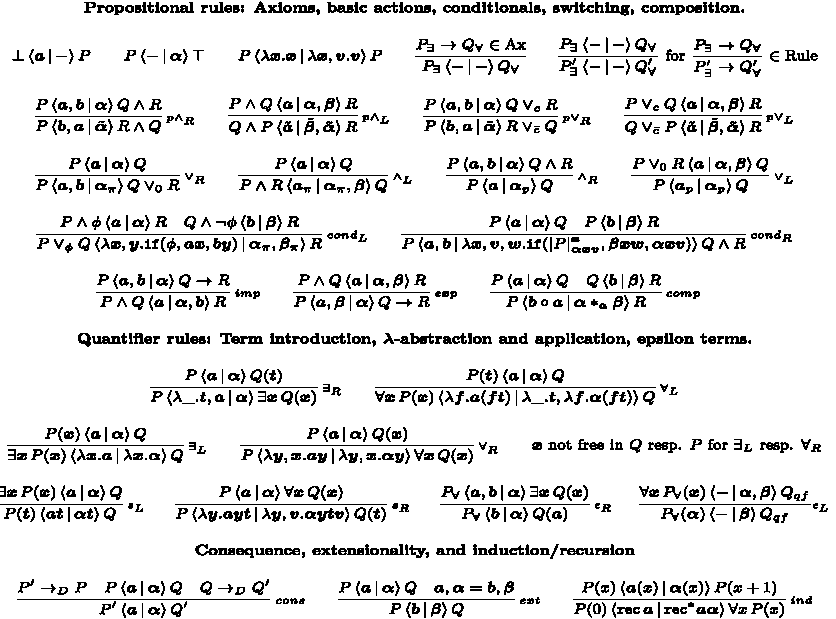
\includegraphics[width=0.95\linewidth,height=0.45\textheight,keepaspectratio]{graphic-01.pdf}\end{center}\par
 
Figure 1: Rules for Dialectica triples, definitions and abbreviations discussed in Section 3.1.\par
 
% END S3.F1
 
% BEGIN S3.SS1.p1
 
It is natural to ask what Hoare-like rules govern Dialectica realizers when viewed in this way. Fixing sets $\mathrm{Ax},\mathrm{Rule}$ of axioms and rules in $\mathrm{WE}\mbox{-}\mathrm{HA}^{\omega}$, we define a judgment system $\mathrm{DHL}$ (for Dialectica Hoare Logic) which derives judgments of shape $P\langle{\bm{a}}\,|\,{\bm{\alpha}}\rangle Q$, where $P,Q$ are formulas of $\mathrm{WE}\mbox{-}\mathrm{HA}^{\omega}$ and $\bm{a},\bm{\alpha}$ are (sequences of) terms of System T, according to the rules in Figure 1. In all cases, the types of $\bm{a},\bm{\alpha}$ are left implicit, but can be inferred from the rules and formulas, as usual in Dialectica. These rules are described in detail in the points below, where we also clarify the notations and abbreviations used.\par
 
% END S3.SS1.p1
 
% BEGIN S3.SS1.p2
  
\par\noindent  $\blacksquare$ 
% BEGIN S3.I1.i1.p1
 
We write $P_{\exists}$ to denote a formula whose Dialectica interpretation is purely existential i.e. of the form $\exists\bm{x}\,|{P}|^{\bm{x}}$. Similarly, $P_{\forall}$ and $P_{qf}$ mean that the Dialectica interpretation of $P$ is purely universal resp. quantifier-free.\par
 
% END S3.I1.i1.p1
 
 
\par\noindent  $\blacksquare$ 
% BEGIN S3.I1.i2.p1
 
The sets $\mathrm{Ax}$ and $\mathrm{Rule}$ denote sets of universal axioms and rules that we add to the system: At the very least $\mathrm{Ax}$ would include the axioms and rules for $=_{\mathsf{nat}}$ along with those governing System T terms, while $\mathrm{Rule}$ would include the quantifier-free extensionality rule, but we leave open the possibility that other axioms and rules could be included.\par
 
% END S3.I1.i2.p1
 
 
\par\noindent  $\blacksquare$ 
% BEGIN S3.I1.i3.p1
 
For $c:\mathsf{nat}$ we define $\bar{c}$ by $\bar{0}:=1$ and $\overline{n+1}:=0$.\par
 
% END S3.I1.i3.p1
 
 
\par\noindent  $\blacksquare$ 
% BEGIN S3.I1.i4.p1
 
$\tilde{\bm{\alpha}}$ denotes a permutation of the arguments of $\bm{\alpha}$, whose precise definition varies but can be immediately inferred from the rule. For example, written out fully, the $\tilde{\bm{\alpha}}$ in the conclusion of $(p\wedge_{R})$ should be $\tilde{\bm{\alpha}}:=\lambda\bm{x},\bm{w},\bm{v}.\bm{\alpha}\bm{x}\bm{v}\bm{w}$ and the intuitive meaning of the triple is the formula $\forall\bm{x},\bm{w},\bm{v}\left(|{P}|^{\bm{x}}_{\tilde{\bm{\alpha}}\bm{x}\bm{w}\bm{v}}\to|{R}|^{\bm{b}\bm{x}}_{\bm{w}}\wedge|{Q}|^{\bm{a}\bm{x}}_{\bm{v}}\right)$. This further illustrates our philosophy on implicit typing: The aim of our notation is to suppress bureaucratic $\lambda$-terms wherever these can be directly inferred.\par
 
% END S3.I1.i4.p1
 
 
\par\noindent  $\blacksquare$ 
% BEGIN S3.I1.i5.p1
 
In a similar way, $\bm{\alpha}_{\pi}$ denotes a projection (e.g. in $(\vee_{R})$, $\bm{\alpha}_{\pi}$ is shorthand for $\lambda\bm{x},\bm{y},\bm{v}.\bm{\alpha}\bm{x}\bm{v}$), while $\bm{\alpha}_{p}$ denotes a coprojection, by which we mean the instantiation of certain arguments with canonical zero terms $\bm{0}$ of the right type (e.g. in $(\wedge_{R})$, $\bm{\alpha}_{p}$ is shorthand for $\lambda\bm{x},\bm{v}.\bm{\alpha}\bm{x}\bm{v}\bm{0}$).\par
 
% END S3.I1.i5.p1
 
 
\par\noindent  $\blacksquare$ 
% BEGIN S3.I1.i6.p1
 
$\lambda\_.t$ denotes the constant term $\lambda\bm{x}.\bm{t}$, where the types of $\bm{x}$, not free in $t$, are to be inferred.\par
 
% END S3.I1.i6.p1
 
 
\par\noindent  $\blacksquare$ 
% BEGIN S3.I1.i7.p1
 
For the conditional rules, $\phi$ is always quantifier-free.\par
 
% END S3.I1.i7.p1
 
 
\par\noindent  $\blacksquare$ 
% BEGIN S3.I1.i8.p1
 
For composition, $\circ$ denotes the usual composition of functions, while $\ast$ denotes the special backwards composition for the Dialectica interpretation, with\par
  
\par  \quad  \[\bm{\alpha}\ast_{\bm{a}}\bm{\beta}:=\lambda\bm{x},\bm{w}.\bm{\alpha}\bm{x}\left(\bm{\beta}(\bm{a}\bm{x})\bm{w}\right)\]\quad  \quad  
  
% END S3.I1.i8.p1
 
 
\par\noindent  $\blacksquare$ 
% BEGIN S3.I1.i9.p1
 
For the quantifier rules we write $Q(\bm{x})$ to denote all occurrences of the free variables $\bm{x}$ in $Q$, and note that there may be no occurrences. We assume the usual rules for substitution e.g. in $(\exists_{R})$ that $\bm{t}$ is free for $\bm{x}$ in $Q$, and similarly for the other rules.\par
 
% END S3.I1.i9.p1
 
 
\par\noindent  $\blacksquare$ 
% BEGIN S3.I1.i10.p1
 
Rule $(cons)$ is the Dialectica version of the usual consequence rules, where the pre- and postconditions can be weakened/strengthened with no bearing on the program. More precisely, we define the $\mathrm{WE}\mbox{-}\mathrm{HA}^{\omega}$-formula $P^{\prime}\to_{D}P$ by\par
  
\par  \quad  \[\forall\bm{x},\bm{v}\left(|{P^{\prime}}|^{\bm{x}}_{\bm{v}}\to|{P}|^{\bm{x}}_{\bm{v}}\right)\]\quad  \quad  
  
i.e. the witnessing types of $P^{\prime}$ and $P$ coincide under the Dialectica and implication is interpreted by the identity.\par
 
% END S3.I1.i10.p1
 
 
\par\noindent  $\blacksquare$ 
% BEGIN S3.I1.i11.p1
 
Finally, $\mathtt{rec}$ denotes the usual recursor whose defining axiom is given in Section 2, while the backward recursor $\mathtt{rec}^{\ast}$ is defined (using the main recursor) as $\mathtt{rec}^{\ast}\bm{a}\bm{\alpha}\bm{y}x\bm{v}:=\bm{\beta}x$ for\par
  
\par  \quad  \[\bm{\beta}0:=\bm{v}\ \ \ \mbox{and}\ \ \ \bm{\beta}(z+1):=\bm{\alpha}(x-z-1)(\mathtt{rec}\,\bm{a}\bm{y}(x-z-1))(\bm{\beta}z).\]\quad  \quad  
  
% END S3.I1.i11.p1
 
  
% END S3.SS1.p2
 
% BEGIN Thmtheorem3
 
\par\medskip\noindent\textbf{Theorem 3.}\par
 
% BEGIN Thmtheorem3.p1
 
Assuming that all elements of $\mathrm{Ax}$ and $\mathrm{Rule}$ are admissible in $\mathrm{WE}\mbox{-}\mathrm{HA}^{\omega}$, if ${P}\,{\langle{\bm{a}}\,|\,{\bm{\alpha}}\rangle}\,{Q}$ is derivable from the rules in Figure 1, then $\forall\bm{x},\bm{v}\left(|{P}|^{\bm{x}}_{\bm{\alpha}\bm{x}\bm{v}}\to|{Q}|^{\bm{a}\bm{x}}_{\bm{v}}\right)$ is provable in $\mathrm{WE}\mbox{-}\mathrm{HA}^{\omega}$.\par
 
% END Thmtheorem3.p1
 
% END Thmtheorem3
 
% BEGIN S3.SS1.p3
 
The proof of Theorem 3 is routine, and involves no ideas fundamentally different to those already present in the usual soundness proofs of Dialectica for $\mathrm{WE}\mbox{-}\mathrm{HA}^{\omega}$. Some of the more interesting rules are discussed in the appendix. We note that by restricting the rules of $\mathrm{DHL}$ so that the precondition is always purely existential, we obtain a simplified set of rules that act only on left-hand realizers, and very closely reflect traditional Hoare rules. These are also presented in the appendix, in Figure 9.\par
 
% END S3.SS1.p3
 
% BEGIN S3.SS1.SSS0.Px1
 
\par\medskip\noindent\textbf{Using $\mathrm{DHL}$}\par
 
% BEGIN S3.F2

\begin{center}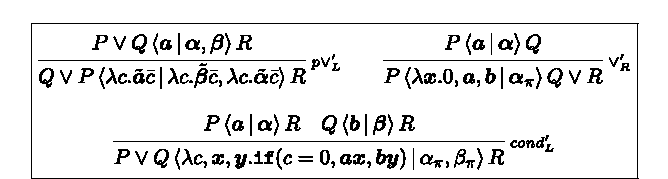
\includegraphics[width=0.95\linewidth,height=0.45\textheight,keepaspectratio]{graphic-02.pdf}\end{center}
 
Figure 2: Rules for disjunction, derivable from those in Figure 1, which can be added to $\mathrm{DHL}$.\par
 
% END S3.F2
 
% BEGIN S3.SS1.SSS0.Px1.p1
 
Our system $\mathrm{DHL}$ is, above all, intended to be a useful system for constructing and describing realizing terms. It is certainly not a minimal system: Indeed, because $(cons)$ ranges over all implications of form $\to_{D}$ derivable in $\mathrm{WE}\mbox{-}\mathrm{HA}^{\omega}$, it can be used together with the quantifier introduction rules to derive all of the others. However, a human (or a machine) using the system would typically use $(cons)$ only in in cases where $P^{\prime}\to_{D}P$ and $Q\to_{D}Q^{\prime}$ are immediate (e.g. have no computational content), and would resort to the main rules for constructing complex terms.\par
 
% END S3.SS1.SSS0.Px1.p1
 
% BEGIN S3.SS1.SSS0.Px1.p2
 
We view the system as fundamentally extendible: The rules in Figure 1 provide the basic manipulations on terms required to show that the Dialectica is sound for $\mathrm{WE}\mbox{-}\mathrm{HA}^{\omega}$, but in practice, especially if we envisage $\mathrm{DHL}$ being incorporated into some proof assistant as a way of reasoning about Dialectica realizers, we would add a range of derivable rules for dealing with specific mathematical structures in proofs, along with new rules for characterising additional constructs added to System T. We give several examples of these in what follows. As a simple illustration, in Figure 2 we note several rules involving disjunction that are easily derivable from those for $\vee_{b}$ along with $(cons)$ and the fact that $P\vee Q\leftrightarrow_{D}\exists b(P\vee_{b}Q)$.\par
 
% END S3.SS1.SSS0.Px1.p2
 
% BEGIN S3.SS1.SSS0.Px1.p3
 
It is now natural to ask: What purely logical system is mirrored by $\mathrm{DHL}$? This can be quite interesting, especially so when we consider extensions to our rules later on. We first note that if we remove $(\epsilon_{L})$, $(\epsilon_{R})$, $(cons)$, $(ext)$ from those of Figure 1, and then replace the disjunction rules with those of Figure 2, these rules can be adapted to form a logical system in the language of $\mathrm{WE}\mbox{-}\mathrm{HA}^{\omega}$ by just suppressing the realizing term. For example, we can simplify the rule $(cond_{L}^{\prime})$ as\par
 
% END S3.SS1.SSS0.Px1.p3
 
% BEGIN S3.SS1.SSS0.Px1.p4
 
\begin{center}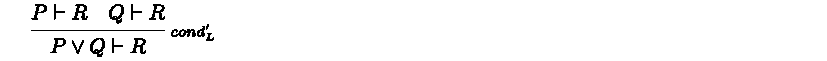
\includegraphics[width=0.95\linewidth,height=0.45\textheight,keepaspectratio]{graphic-03.pdf}\end{center}
 
% END S3.SS1.SSS0.Px1.p4
 
% BEGIN S3.SS1.SSS0.Px1.p5
 
and similarly for the others. Letting $\mathcal{H}$ denote the resulting system, we have the following:\par
 
% END S3.SS1.SSS0.Px1.p5
 
% BEGIN Thmtheorem4
 
\par\medskip\noindent\textbf{Theorem 4.}\par
 
% BEGIN Thmtheorem4.p1
 
Whenever $P$ is provable in $\mathrm{WE}\mbox{-}\mathrm{HA}^{\omega}$, then $\top\vdash P$ is provable in $\mathcal{H}$.\par
 
% END Thmtheorem4.p1
 
% END Thmtheorem4
 
% BEGIN S3.SS1.SSS0.Px1.p6
 
Again, the proof is straightforward, and a rough sketch of how we show this is provided in the appendix. Theorem 4 therefore represents an alternative soundness proof from the Dialectica interpretation of $\mathrm{WE}\mbox{-}\mathrm{HA}^{\omega}$, and another way of using $\mathrm{DHL}$: If $P$ is provable in $\mathrm{WE}\mbox{-}\mathrm{HA}^{\omega}$, we take an alternative derivation of $\top\vdash P$ in $\mathcal{H}$ and adding back the hidden realizing terms we obtain a derivation of\par
  
\par  \quad  \[{\top}\,{\langle{\bm{a}}\,|\,{-}\rangle}\,{P}=\forall\bm{v}|{P}|^{\bm{a}}_{\bm{v}}\]\quad  \quad  
  
where $\bm{a}$ is constructed via the derivation (note that we can also force that the free variables of $\bm{a}$ are contained in those of $P$ by applying $(\exists_{L})$ on all superfluous variables and then $(s_{L})$ instantiated with zero terms). We also observe that if $P\to Q$ is any formula such that $P\leftrightarrow_{D}R\leftrightarrow_{D}Q$ for some suitable $R$, then ${P}\,{\langle{\lambda\bm{x}.\bm{x}}\,|\,{\lambda\bm{x},\bm{v}.\bm{v}}\rangle}\,{Q}$ is immediately derivable from the $(cons)$ rule and therefore $P\vdash Q$ can be added to $\mathcal{H}$. In this way, we also regain that $\mathrm{AC}$, $\mathrm{IP}^{\omega}_{\forall}$ and $\mathrm{M}^{\omega}$ are admissible by the Dialectica.\par
 
% END S3.SS1.SSS0.Px1.p6
 
% BEGIN S3.SS1.SSS0.Px1.p7
 
There are still three rules we have not discussed. While $(ext)$ is just an extensionality rule purely for reasoning about extracted terms, $(\epsilon_{L})$ and $(\epsilon_{R})$ are more interesting. These essentially allow us access to epsilon terms: Informally speaking, we can add these rules to our purely logical system $\mathcal{H}$ as\par
 
% END S3.SS1.SSS0.Px1.p7
 
% BEGIN S3.SS1.SSS0.Px1.p8
 
\begin{center}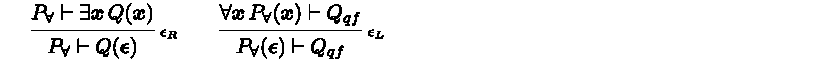
\includegraphics[width=0.95\linewidth,height=0.45\textheight,keepaspectratio]{graphic-04.pdf}\end{center}
 
% END S3.SS1.SSS0.Px1.p8
 
% BEGIN S3.SS1.SSS0.Px1.p9
 
where here we would add a countable set of epsilon terms $(\epsilon_{i})$ to our language and use a fresh sequence of $\epsilon$-terms for each instance of $(\epsilon_{L})$, $(\epsilon_{R})$ in a derivation. The hidden realizing terms allow us to always assign concrete values to these $\epsilon$-terms, which can then be substituted in should any remain at the end of a derivation. However, some care is needed to set this up formally. Interestingly, the addition of $\epsilon$-terms to intuitionistic logic is explored in [23]: There, doing this for arbitrary formulas does not give us a conservative extension of intuitionistic logic, as the full independence of premise axiom is then derivable222We are grateful to Cameron Allett for directing us to [23].. Our in-built restriction for $(\epsilon_{R})$ that the left hand formula has purely universal Dialectica interpretation avoids this problem: We are then only able to derive independence of premise for universal formulas, and this is admissible by Dialectica!\par
 
% END S3.SS1.SSS0.Px1.p9
 
% BEGIN S3.SS1.SSS0.Px1.p10
 
Finally, we note that by taking advantage of the infrastructure is already available via Oliva’s unified approach to functional interpretations [30], it would not be hard to parametrise our own system $\mathrm{DHL}$ with abstract bounding relation $\sqsubset$ and thereby obtain both the traditional Dialectica, modified realizability and the Diller-Nahm interpretation [10] as instances. For the latter, the conditional rule $(cond_{R})$ would then look like\par
 
% END S3.SS1.SSS0.Px1.p10
 
% BEGIN S3.SS1.SSS0.Px1.p11
 
\begin{center}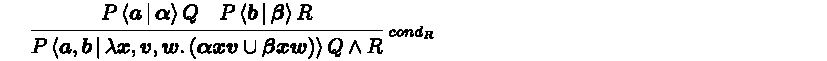
\includegraphics[width=0.95\linewidth,height=0.45\textheight,keepaspectratio]{graphic-05.pdf}\end{center}
 
% END S3.SS1.SSS0.Px1.p11
 
% BEGIN S3.SS1.SSS0.Px1.p12
 
for $\cup$ a union operation on finite sets.\par
 
% END S3.SS1.SSS0.Px1.p12
 
% END S3.SS1.SSS0.Px1
 
% END S3.SS1
 
% BEGIN S3.SS2
 
\par\medskip\noindent\textbf{3.2 A while rule for Dialectica, and its use in classical logic}\par
 
% BEGIN S3.SS2.p1
 
We characterised $\mathrm{DHL}$ as being inspired by Hoare logic, but conspicuously absent so far are any kind of imperative control flow statements. To that end, we introduce a while construct and identify a corresponding rule that is sound in our base system. We argue that in the context of Dialectica, this while loop is well-suited to describing how programs extracted from classical logic implement “learning algorithms”.\par
 
% END S3.SS2.p1
 
% BEGIN S3.SS2.p2
 
For the present paper, we restrict our attention to programs that are total, so our while rule is specified relative to some wellfounded relation. We first introduce a decidable binary relation $\prec$ on objects of type $\bm{X}$, which can be modelled in $\mathrm{WE}\mbox{-}\mathrm{HA}^{\omega}$ as a function $\prec:\bm{X}\to\bm{X}\to\mathsf{nat}$. We then expand $\mathrm{WE}\mbox{-}\mathrm{HA}^{\omega}$ with a wellfounded induction rule $\mathrm{I}_{\prec}$ given by\par
 
% END S3.SS2.p2
 
% BEGIN S3.SS2.p3
 
\begin{center}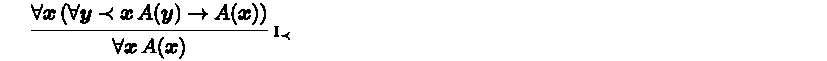
\includegraphics[width=0.95\linewidth,height=0.45\textheight,keepaspectratio]{graphic-06.pdf}\end{center}
 
% END S3.SS2.p3
 
% BEGIN S3.SS2.p4
 
where $A(\bm{x})$ ranges over arbitrary formulas. Now, for a quantifier-free formula $\phi(\bm{x}^{\bm{X}})$ and a term $\bm{a}:\bm{X}\to\bm{X}$, for any sequence of types $\bm{U}$ we add to the language of $\mathrm{WE}\mbox{-}\mathrm{HA}^{\omega}$ a while recursor $\mathtt{whilerec}_{\prec,\phi,\bm{a}}:(\bm{X}\to\bm{U})\to(\bm{X}\to\bm{U}\to\bm{U})\to\bm{X}\to\bm{U}$ along with the schema\par
  
\par  \quad  \[(\phi(\bm{x})\to\bm{a}\bm{x}\prec\bm{x})\to\mathtt{whilerec}_{\prec,\phi,\bm{a}}\bm{u}\bm{F}\bm{x}=_{\bm{U}}\mathtt{if}({\phi(\bm{x})},{\bm{F}\bm{x}\left(\mathtt{whilerec}_{\prec,\phi,\bm{a}}\bm{u}\bm{F}(\bm{a}\bm{x})\right)},{\bm{u}\bm{x}})\]\quad  \quad  
  
where here the premise ensures that triggering the condition of the while loop causes a descent along $\prec$. We write $\mathrm{WE}\mbox{-}\mathrm{HA}^{\omega}+(\mathtt{whilerec}_{\prec})$ for $\mathrm{WE}\mbox{-}\mathrm{HA}^{\omega}$ extended with the while recursor and its axiom for all $\phi$ and $\bm{a}$. Now we define the forward while operator $\mathtt{while}^{+}_{\prec}\,{\phi}\,\mathtt{do}\,{\bm{a}}:\bm{X}\to\bm{X}$ as\par
  
\par  \quad  \[\mathtt{while}^{+}_{\prec}\,{\phi}\,\mathtt{do}\,{\bm{a}}:=\mathtt{whilerec}_{\prec,\phi,\bm{a}}(\lambda\bm{x}.\bm{x})(\lambda\bm{x},\bm{y}.\bm{y})\]\quad  \quad  
  
and the backward operator $\mathtt{while}^{-}_{\prec}\,{\phi}\,\mathtt{do}\,{(\bm{a},\bm{\alpha})}:\bm{X}\to\bm{V}\to\bm{V}$ for $\bm{\alpha}:\bm{X}\to\bm{V}\to\bm{V}$ as\par
  
\par  \quad  \[\mathtt{while}^{-}_{\prec}\,{\phi}\,\mathtt{do}\,{(\bm{a},\bm{\alpha})}:=\mathtt{whilerec}_{\prec,\phi,\bm{a}}(\lambda\bm{x},\bm{v}.\bm{v})(\lambda\bm{x},\bm{f},\bm{v}.\bm{\alpha}\bm{x}(\bm{f}\bm{v})).\]\quad  \quad  
  
The following result, easily proven by expanding the definitions, guarantees that the forward while behaves indeed as a while loop. The backward direction is more subtle, and we discuss how it can be interpreted as part of a stateful program in Section 4.\par
 
% END S3.SS2.p4
 
% BEGIN Thmtheorem5
 
\par\medskip\noindent\textbf{Lemma 5.}\par
 
% BEGIN Thmtheorem5.p1
 
Whenever $\phi(\bm{x})\to\bm{a}\bm{x}\prec\bm{x}$ is provable in $\mathrm{WE}\mbox{-}\mathrm{HA}^{\omega}$, the following are provable in $\mathrm{WE}\mbox{-}\mathrm{HA}^{\omega}+(\mathtt{whilerec}_{\prec})$:\par
  
\par  \quad  \quad  $\displaystyle(\mathtt{while}^{+}_{\prec}\,{\phi}\,\mathtt{do}\,{\bm{a}})\bm{x}=\mathtt{if}({\phi(\bm{x})},{(\mathtt{while}^{+}_{\prec}\,{\phi}\,\mathtt{do}\,{\bm{a}})(\bm{a}\bm{x})},{\bm{x}}),$\quad  \quad  
 
\par  \quad  \quad  $\displaystyle(\mathtt{while}^{-}_{\prec}\,{\phi}\,\mathtt{do}\,{(\bm{a},\bm{\alpha})})\bm{x}\bm{v}=\mathtt{if}({\phi(\bm{x})},{\bm{\alpha}\bm{x}\left((\mathtt{while}^{-}_{\prec}\,{\phi}\,\mathtt{do}\,{(\bm{a},\bm{\alpha})})(\bm{a}\bm{x})\bm{v}\right)},{\bm{v}}).$\quad  \quad  
  
% END Thmtheorem5.p1
 
% END Thmtheorem5
 
% BEGIN S3.SS2.p5
 
We now define a corresponding rule for any decidable relation $\prec$, namely\par
 
% END S3.SS2.p5
 
% BEGIN S3.SS2.p6
 
\begin{center}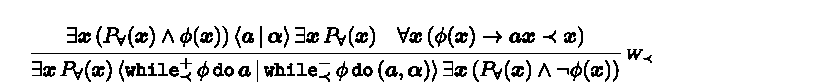
\includegraphics[width=0.95\linewidth,height=0.45\textheight,keepaspectratio]{graphic-07.pdf}\end{center}
 
% END S3.SS2.p6
 
% BEGIN S3.SS2.p7
 
The rule $W_{\prec}$ is closely connected to the wellfounded while rule of Hoare logic, with the difference that the descent condition is now presented separately. The following result (proven in the appendix) connects the rule to the recursor, and bears some relationship to the interpretation of wellfounded induction in [38].\par
 
% END S3.SS2.p7
 
% BEGIN Thmtheorem6
 
\par\medskip\noindent\textbf{Theorem 6.}\par
 
% BEGIN Thmtheorem6.p1
 
The while rule $(W_{\prec})$ is admissible in $\mathrm{WE}\mbox{-}\mathrm{HA}^{\omega}+\mathrm{I}_{\prec}+(\mathtt{whilerec}_{\prec})$.\par
 
% END Thmtheorem6.p1
 
% END Thmtheorem6
 
% BEGIN S3.SS2.SSS0.Px1
 
\par\medskip\noindent\textbf{Discussion: The interpretation of classical logic and its interaction with $\mathtt{whilerec}_{\prec}$}\par
 
% BEGIN S3.F3

\begin{center}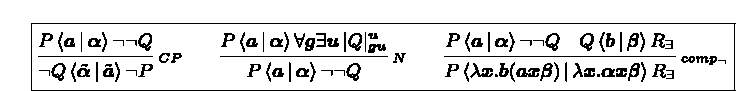
\includegraphics[width=0.95\linewidth,height=0.45\textheight,keepaspectratio]{graphic-08.pdf}\end{center}
 
Figure 3: Example rules for manipulating classical proofs under the double negation translation.\par
 
% END S3.F3
 
% BEGIN S3.SS2.SSS0.Px1.p1
 
It is well known that classical logic can be given a computational interpretation via the Dialectica by first carrying out a negative translation (see [18, Chapter 10]), where the embedding of classical logic into intuitionistic makes use of a number of (semi-intuitionistic) laws governing negations. Expanding $\mathrm{DHL}$ with these laws as primitives would allow for a streamlined verification of programs extracted from classical proofs, and though detailed exploration of this is beyond the scope of the present paper, we give three examples of the kind of rules we have in mind, in Figure 3.\par
 
% END S3.SS2.SSS0.Px1.p1
 
% BEGIN S3.SS2.SSS0.Px1.p2
 
Here, $(CP)$ and $(N)$ are extremely useful (and reversible) symmetry rules that one often encounters when analysing classical proofs, while $(comp_{\neg})$ is a version of composition which illustrates one way in which the negative translation composed with Dialectica eliminates nonconstructive lemmas when proving purely existential formulas, as we discuss below.\par
 
% END S3.SS2.SSS0.Px1.p2
 
% BEGIN S3.F4
 
\begin{center}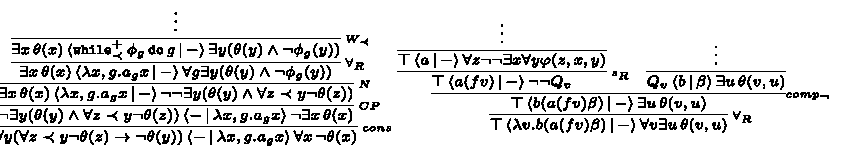
\includegraphics[width=0.95\linewidth,height=0.45\textheight,keepaspectratio]{graphic-09.pdf}\end{center}\par
 
Figure 4: Left: For $g:X\to X$ we use the abbreviation $\phi_{g}(x):=gx\prec x\wedge\theta(gx)$ and $a_{g}:=\mathtt{while}^{+}_{\prec}\,{\phi_{g}}\,\mathtt{do}\,{g}$. One completes the derivation by using ${\exists x(\theta(x)\wedge\phi_{g}(x))}\,{\langle{g}\,|\,{-}\rangle}\,{\exists
y\,\theta(y)}$ and $\forall x(\phi_{g}(x)\to gx\prec x)$, which are easily provable. Right: we use the negative translation to obtain a constructive proof of the double negated statement that appears in the left branch.\par
 
% END S3.F4
 
% BEGIN S3.SS2.SSS0.Px1.p3
 
An example of how our while rule in particular interacts with these new principles for handling double negation is given on the left side of Figure 4, where we use it to define a realiser for double-negated version of the following minimum principle:\par
  
\par  \quad  \[\exists x\,\theta(x)\vdash\exists x\left(\theta(x)\wedge\forall y\prec x\neg\theta(y)\right),\]\quad  \quad  
  
where $\theta(x^{X})$ is a quantifier-free formula and $\prec$ is a wellfounded relation on $X$ (we omit simple instances of $(ext)$ to improve readability). This represents a derivation, in a Hoare style system, of the kind of intuitive algorithm for the minimum principle already described in e.g. [6, Section 7], and the imperative flavour of such constructions in relation to the Dialectica interpretation is also discussed in [34], where an explicit connection to learning algorithms is drawn. This general phenomenon of computing approximations to ideal objects via learning is present in almost all approaches to giving a computational meaning to classical reasoning: the epsilon calculus, modified realizability [7], game semantics [6], approaches based on learning [2], the $\lambda\mu$-calculus [32], call-cc [13], classical realizability [22, 24] and others (see [35] for a comparative study of some of these), and we propose that our approach via Hoare logic might help make explicit this intuition in the context of Dialectica.\par
 
% END S3.SS2.SSS0.Px1.p3
 
% BEGIN S3.SS2.SSS0.Px1.p4
 
Another example where we see our rules for classical logic in action is given by the frequently occurring proof pattern where an instance of a nonconstructive principle is eliminated by the Dialectica when used as a lemma in the proof of a $\forall\exists$-theorem. More precisely, suppose that we establish $\forall v\exists u\,\theta(v,u)$ by showing (constructively) that for any $v$ we have $\exists x\forall y\,\varphi(fv,x,y)\to\exists u\,\theta(v,u),$ for some function $f$, but where the premise is an instance of a principle only provable nonconstructively; for instance, $x$ might be a minimal element in some set, a maximal ideal, or a point after which a sequence is $2^{-fv}$ stable. Abbreviating $\exists x\forall y\,\varphi(fv,x,y)$ with $Q_{v}$, the derivation on the right in Figure 4 provides a basic template for eliminating this nonconstructive principle via $(comp_{\neg})$, combining a witness $a$ for the classical Dialectica interpretation of the latter with a realizing pair for the constructive implication above. There are many cases where the witness $a$ for the double negated lemma could be built in a natural way via using our while loop, against some “counterexample function” provided by the backward witness $\beta$. It might then form a core component of a procedural-style program for computing a witness for $\forall v\exists u\,\theta(v,u)$.\par
 
% END S3.SS2.SSS0.Px1.p4
 
% END S3.SS2.SSS0.Px1
 
% END S3.SS2
 
% END S3


% BEGIN S4
 
\par\medskip\noindent\textbf{4 A procedural language for Dialectica}\par
 
% BEGIN S4.p1
 
So far, we have put forward the argument that having a rich library of rules for Dialectica triples, including imperative constructs like the while loop, is beneficial for describing programs naturally arising from mathematics in a procedural way. In this section, we consider this aspect of our system in a more formal manner. For now we consider a restricted system that aligns closely with traditional Hoare logic, comprising a small set of rules for generating “stateful” programs. Because these rules arise from the Dialectica interpretation, the result is a novel procedural language with nonstandard interpretation. To be more precise, we define a language $\mathrm{LOOP}_{D}$, representing a Dialectica-like extension of a toy procedural language $\mathrm{LOOP}$, and provide both a Hoare logic and an operational semantics, where the latter captures the idea that\par
  
\par  \quad  \[\mathrm{LOOP}_{D}=\mathrm{LOOP}+\text{backpropagation},\]\quad  \quad  
  
i.e. commands of the language consist of an ordinary forward part, together with a backward component that can be computed via a generalised form of backpropagation. We anticipate that this operational semantics that could eventually be extended to our entire system $\mathrm{DHL}$.\par
 
% END S4.p1
 
% BEGIN S4.p2
 
In order to define $\mathrm{LOOP}_{D}$ and its corresponding logic, we extend our ambient theory $\mathrm{WE}\mbox{-}\mathrm{HA}^{\omega}$ with two new abstract types $S$ and $T$ representing two sorts of state. The extension of $\mathrm{WE}\mbox{-}\mathrm{HA}^{\omega}$ with abstract types is standard in the proof mining literature (see [17]), where those types are typically used to represent abstract spaces from mathematics. We then extend the terms $\mathrm{WE}\mbox{-}\mathrm{HA}^{\omega}$ by introducing:\par
  
\par\noindent  $\blacksquare$ 
% BEGIN S4.I1.i1.p1
 
two equality symbols $=_{S}$ and $=_{T}$, which we write as predicates but which will technically be terms $=_{S}:S\to S\to\mathsf{nat}$ and $=_{T}:T\to T\to\mathsf{nat}$ (indicating that equality between states is a decidable property). In addition, we extend all the usual constructs of $\mathrm{WE}\mbox{-}\mathrm{HA}^{\omega}$ e.g. quantifiers, recursors, lambda abstraction, so that they apply to our new states;\par
 
% END S4.I1.i1.p1
 
 
\par\noindent  $\blacksquare$ 
% BEGIN S4.I1.i2.p1
 
two sets of primitive command, the set $\mathtt{Comm}^{+}$ of forward commands of type $S\to S$, and the set $\mathtt{Comm}^{-}$ of backward commands of type $S\to T\to T$;\par
 
% END S4.I1.i2.p1
 
 
\par\noindent  $\blacksquare$ 
% BEGIN S4.I1.i3.p1
 
a set $\mathtt{Exp}$ of boolean expressions, which are formally a set of decidable predicates on $S$ represented in $\mathrm{WE}\mbox{-}\mathrm{HA}^{\omega}$ as characteristic functions of type $S\to S\to\mathsf{nat}$;\par
 
% END S4.I1.i3.p1
 
 
\par\noindent  $\blacksquare$ 
% BEGIN S4.I1.i4.p1
 
a set $\mathtt{Rel}$ of wellfounded relations on $S$.\par
 
% END S4.I1.i4.p1
 
  
% END S4.p2
 
% BEGIN S4.p3
 
We also assume that we have a set of purely universal axioms $\mathcal{U}$ that characterise the meaning of commands and expressions. We then define the set $\mathtt{Comm}$ of commands of $\mathrm{LOOP}_{D}$ as follows, all of which represent new constants or term forming operations in $\mathrm{WE}\mbox{-}\mathrm{HA}^{\omega}$ for generating pairs of terms of types $S\to S,S\to T\to T$:\par
  
\par  \quad  \[C::=\mathtt{skip}\mid\langle{c}\,|\,{\gamma}\rangle\mid{C}\,;\,{C}\mid\mathtt{if}\,{\phi}\,\mathtt{then}\,{C}\,\mathtt{else}\,{C}\mid\mathtt{while}_{\prec}\,{\phi}\,\mathtt{do}\,{C}\]\quad  \quad  
  
where $c\in\mathtt{Comm}^{+}$, $\gamma\in\mathtt{Comm}^{-}$, $\phi\in\mathtt{Exp}$ and $\prec\in\mathtt{Rel}$.\par
 
% END S4.p3
 
% BEGIN S4.F5
   
\par  \quad  \[\begin{array}[]{|c|c|c|}\hline\cr\mathrm{LOOP}_{D}&(\_)^{+}&(\_)^{-}\\
\hline\cr\mathtt{skip}&\lambda s.s&\lambda s,t.t\\[1.99168pt]
\langle{c}\,|\,{\gamma}\rangle&c&\gamma\\[1.99168pt]
{C_{1}}\,;\,{C_{2}}&C_{2}^{+}\circ C_{1}^{+}&C_{1}^{-}\ast_{C_{1}^{+}}C_{2}^{-}\\[1.99168pt]
\mathtt{if}\,{\phi}\,\mathtt{then}\,{C_{1}}\,\mathtt{else}\,{C_{2}}&\lambda s.\mathtt{if}({\phi(s)},{C^{+}_{1}s},{C^{+}_{2}s})&\lambda s,t.\mathtt{if}({\phi(s)},{C^{-}_{1}st},{C^{-}_{2}st})\\[1.99168pt]
\mathtt{while}_{\prec}\,{\phi}\,\mathtt{do}\,{C}&\mathtt{while}^{+}_{\prec}\,{\phi}\,\mathtt{do}\,{C^{+}}&\mathtt{while}^{-}_{\prec}\,{\phi}\,\mathtt{do}\,{(C^{+},C^{-})}\\
\hline\cr\end{array}\]\quad  \quad  
   
Figure 5: Decomposition in $\mathrm{WE}\mbox{-}\mathrm{HA}^{\omega}$ of $\mathrm{LOOP}_{D}$ terms in System T terms. Remember the Dialectica composition $\ast$ from Section 3 and the while constructors from Section 3.2.\par
 
% END S4.F5
 
% BEGIN S4.p4
 
The new constructors come equipped with the defining axiom\par
  
\par  \quad  \[C=\langle{C^{+}}\,|\,{C^{-}}\rangle,\]\quad  \quad  
  
where $\langle{}\,|\,{}\rangle$ is a fixed representation of pairs in $\mathrm{WE}\mbox{-}\mathrm{HA}^{\omega}$ and $C^{+}:S\to S$ and $C^{-}:S\to T\to T$ are defined inductively over $\mathtt{Comm}$ as in Figure 5. In particular, notice that by Lemma 5 we have that if $\neg\phi(s)$, then $(\mathtt{while}_{\prec}\,{\phi}\,\mathtt{do}\,{C_{1}})s=(\mathtt{skip})s$, and whenever $\phi(s)$ and $C^{+}s\prec s$, then\par
  
\par  \quad  \[(\mathtt{while}_{\prec}\,{\phi}\,\mathtt{do}\,{C})s=({C}\,;\,{\mathtt{while}_{\prec}\,{\phi}\,\mathtt{do}\,{C}})s.\]\quad  \quad  
  
We denote by $\mathrm{WE}\mbox{-}\mathrm{HA}^{\omega}+(\mathrm{LOOP}_{D})$ the extension of $\mathrm{WE}\mbox{-}\mathrm{HA}^{\omega}$ with all of the above (including the while recursor and well-founded induction axiom for all $\prec\in\mathtt{Rel}$).\par
 
% END S4.p4
 
% BEGIN S4.F6
 
\begin{center}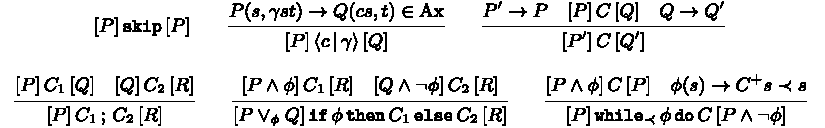
\includegraphics[width=0.95\linewidth,height=0.45\textheight,keepaspectratio]{graphic-10.pdf}\end{center}\par
 
Figure 6: Hoare rules for Dialectica triples in $\mathrm{LOOP}_{D}$. Notice that we use some abbreviations: $P\wedge\phi$ is sugar for the formula $P(s,t)\wedge\phi(s)$, and $P\vee_{\phi}Q$ for the formula $P(s,t)\vee_{\phi(s)}Q(s,t)$.\par
 
% END S4.F6
 
% BEGIN S4.p5
 
Figure 5 characterises our commands as comprising a standard imperative forward part, with a “Dialectica version” of the same component as the backward part. A corresponding set of specification rules is now given in terms of our Dialectica triples in Figure 6: Here we use the more compact and suggestive abbreviation\par
  
\par  \quad  \[[{P}]\,{C}\,[{Q}]:={\exists s\forall t\,P(s,t)}\,{\langle{C^{+}}\,|\,{C^{-}}\rangle}\,{\exists s\forall t\,Q(s,t)}=\forall s,t\left(P(s,C^{-}st)\to Q(C^{+}s,t)\right)\]\quad  \quad  
  
and restrict our attention to Dialectica triples whose pre- and postconditions are formulas of the form $\exists s^{S}\forall t^{T}\,P(s,t)$ where $P(s,t)$ is quantifier-free, and $s,t$ are the only free variables of type $S,T$ that appear in them. In the second rule, $\mathrm{Ax}$ represents some set of axioms that govern the primitive commands, which we assume are included in $\mathcal{U}$. All of these rules are either instances of the main rules from previous sections, or in the case of conditional, easily derivable, and so it is straightforward to prove the following:\par
 
% END S4.p5
 
% BEGIN Thmtheorem7
 
\par\medskip\noindent\textbf{Theorem 7.}\par
 
% BEGIN Thmtheorem7.p1
 
All rules in Figure 6 are admissible in $\mathrm{WE}\mbox{-}\mathrm{HA}^{\omega}+(\mathrm{LOOP}_{D})$.\par
 
% END Thmtheorem7.p1
 
% END Thmtheorem7
 
% BEGIN S4.p6
 
We also note that Figure 6 only shows one set of rules corresponding to traditional Hoare logic: Plenty more are admissible (e.g. those for conjunction and disjunction).\par
 
% END S4.p6
 
% BEGIN S4.SS0.SSS0.Px1
 
\par\medskip\noindent\textbf{An operational semantics for $\mathrm{LOOP}_{D}$ via backpropagation}\par
 
% BEGIN S4.F7

\begin{center}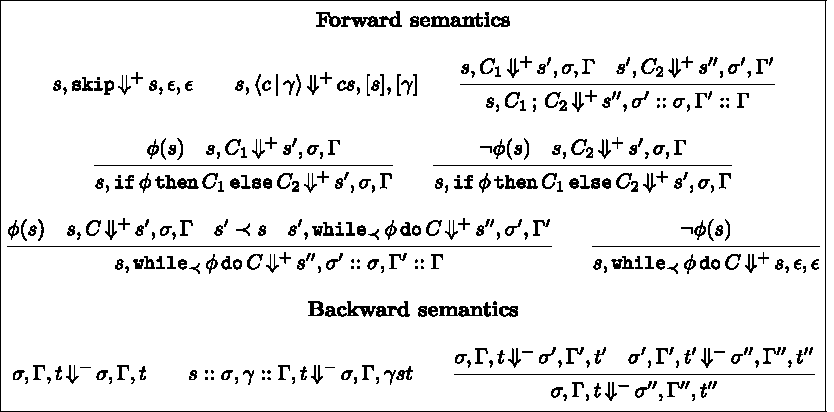
\includegraphics[width=0.95\linewidth,height=0.45\textheight,keepaspectratio]{graphic-11.pdf}\end{center}
 
Figure 7: Operational semantics for $\mathrm{LOOP}_{D}$.\par
 
% END S4.F7
 
% BEGIN S4.SS0.SSS0.Px1.p1
 
So far, $\mathrm{LOOP}_{D}$ is just an extension of System T, with equational rules that describe the meaning of terms. We now endow terms of $\mathrm{LOOP}_{D}$ with a big step operational semantics, to highlight how they can be interpreted as “stateful” programs. We first introduce some notation: For any type $X$ we let $X^{\ast}$ denote the type of finite sequences of elements of $X$ (while this is not formally part of $\mathrm{WE}\mbox{-}\mathrm{HA}^{\omega}$, it can easily be encoded in the system, though we omit details). For $\sigma,\tau:X^{\ast}$ we write $\tau::\sigma:X^{\ast}$ for the concatenation of two sequences, and for $x:X$ similarly write $x::\sigma$ for concatenation with a single element. We write $\epsilon$ for the empty list (of any type). Our semantics comprises two components: A forward relation and a backward relation, which we write\par
  
\par  \quad  \[{s},{C}\,{\Downarrow^{+}}\,{s^{\prime}},{\sigma},{\Gamma}\ \ \ \mbox{and}\ \ \ {\sigma},{\Gamma},{t}\,{\Downarrow^{-}}\,{\sigma^{\prime}},{\Gamma^{\prime}},{t^{\prime}}\]\quad  \quad  
  
for $s,s^{\prime}:S$, $t,t^{\prime}:T$, $C\in\mathtt{Comm}$, $\sigma,\sigma^{\prime}:S^{\ast}$ and $\Gamma,\Gamma^{\prime}:(S\to T\to T)^{\ast}$. Rules for the semantics are given in Figure 7. If we ignore the stacks, our forward semantics is isomorphic to a standard operational semantics for an imperative language. It is not difficult to show that semantics is sound with respect to the denotational semantics of $\mathrm{WE}\mbox{-}\mathrm{HA}^{\omega}+(\mathrm{LOOP}_{D})$:\par
 
% END S4.SS0.SSS0.Px1.p1
 

% BEGIN Thmtheorem8
 
\par\medskip\noindent\textbf{Theorem 8.}\par
 
% BEGIN Thmtheorem8.p1
 
Let $C$ be an arbitrary command in $\mathrm{LOOP}_{D}$, where we restrict the formation of $\mathtt{while}_{\prec}\,{\phi}\,\mathtt{do}\,{C_{1}}$ to commands such that $\forall s(\phi(s)\to C_{1}^{+}s\prec s)$ is provable in $\mathrm{WE}\mbox{-}\mathrm{HA}^{\omega}$. Then for any $s$ there exist $s^{\prime}$, $\sigma$ and $\Gamma$ such that\par
  
\par  \quad  \[{s},{C}\,{\Downarrow^{+}}\,{s^{\prime}},{\sigma},{\Gamma}\]\quad  \quad  
  
where $s^{\prime}=C^{+}s$ in $\mathrm{WE}\mbox{-}\mathrm{HA}^{\omega}$, and such that for any $t:T$, $\sigma_{0}$ and $\Gamma_{0}$ there exists $t^{\prime}$ such that\par
  
\par  \quad  \[{\sigma::\sigma_{0}},{\Gamma::\Gamma_{0}},{t}\,{\Downarrow^{-}}\,{\sigma_{0}},{\Gamma_{0}},{t^{\prime}}\]\quad  \quad  
  
where $t^{\prime}=C^{-}st$ in $\mathrm{WE}\mbox{-}\mathrm{HA}^{\omega}$.\par
 
% END Thmtheorem8.p1
 
% END Thmtheorem8

 
% BEGIN S4.SS0.SSS0.Px1.p2
 
A proof of Theorem 8 can be found in the appendix. Our operational semantics captures the idea that to evaluate a command $C$ in state $s$, we perform a forward run\par
  
\par  \quad  \[{s},{C}\,{\Downarrow^{+}}\,{s_{k}},{[s_{k-1},\ldots,s_{1},s]},{[\gamma_{k},\ldots,\gamma_{1}]}\]\quad  \quad  
  
where for each $j=1,\ldots,k$ we have $s_{j}=c_{j}s_{j-1}$ for $\langle{c_{j}}\,|\,{\gamma_{j}}\rangle$ a primitive command, and $s_{k}=(c_{k}\circ\ldots\circ c_{1})s=C^{+}s$. In other words, each time we are confronted with a primitive command $\langle{c_{j}}\,|\,{\gamma_{j}}\rangle$ in some intermediate state $s_{j-1}$, we perform the forward component but push both the intermediate state $s_{j-1}$ and the backward command $\gamma_{j}$ onto stacks. The backward run then just pops the intermediate states and commands, with\par
  
\par  \quad  \[{[s_{k-1},\ldots,s_{1},s]},{[\gamma_{k},\ldots,\gamma_{1}]},{t}\,{\Downarrow^{-}}\,{\epsilon},{\epsilon},{(\gamma_{1}s\circ\ldots\circ\gamma_{k}s_{k-1})t}\]\quad  \quad  
  
where $(\gamma_{1}s\circ\ldots\circ\gamma_{k}s_{k-1})t=C^{-}st$ In this way, programs in $\mathrm{LOOP}_{D}$ combine a generalised backpropagation algorithm, where in addition to composing functions we can also perform conditionals and loops. The fact that Dialectica is tightly related with manipulations of stacks in a “backward way” has been discovered in [33], therefore it is not a surprise that stacks also play an essential role in our framework.\par
 
% END S4.SS0.SSS0.Px1.p2
 
% END S4.SS0.SSS0.Px1
 
% BEGIN S4.SS0.SSS0.Px2
 
\par\medskip\noindent\textbf{Discussion: On automatic differentiation}\par
 
% BEGIN S4.SS0.SSS0.Px2.p1
 
The basic connection between Dialectica and backpropagation is not new: In particular, it was explored in the specific context of differentiation in [16]. We can phrase it within our framework as well: Suppose that our state $S$ represent some space on which we can define functions $c:S\to S$ and we have the notion of a differentials $D_{s}({c}):S\to S$ at points $s:S$. Suppose that we can also express the reverse differentials $D^{\ast}_{s}({c}):T\to T$ on the dual space $T$, defined by $D^{\ast}_{s}({c})t:=t\circ D_{s}({c})$. Then for a pair $c_{1},c_{2}:S\to S$ of differentiable functions, it is well-known that we have the transpose version of the chain rule:\par
  
\par  \quad  \[D^{\ast}_{s}({c_{1}})\circ\left(D^{\ast}_{c_{1}(s)}({c_{2}})\right)\]\quad  \quad  
  
or, to put it another way,\par
  
\par  \quad  \[\langle{c_{2}\circ c_{1}}\,|\,{D^{\ast}_{(\cdot)}({c_{2}\circ c_{1}})}\rangle={\langle{c_{1}}\,|\,{D^{\ast}_{(\cdot)}({c_{1}})}\rangle}\,;\,{\langle{c_{2}}\,|\,{D^{\ast}_{(\cdot)}({c_{2}})}\rangle}.\]\quad  \quad  
  
Therefore, if our primitive commands consist of pairs $\langle{c}\,|\,{\gamma}\rangle$ with the property that $\gamma s=D^{\ast}_{s}({c})$, this property is preserved under composition of commands, and the resulting semantics (restricted to composition) gives a version of the traditional backpropagation algorithm.\par
 
% END S4.SS0.SSS0.Px2.p1
 
% BEGIN S4.SS0.SSS0.Px2.p2
 
It should be stressed that our approach is not intended to equate the investigations around Dialectica and differentiation as done in [16], where among other things a precise translation into the differential $\lambda$-calculus is provided. In a certain sense, our presentation is orthogonal, presenting a general backpropagation procedure connected to imperative commands. Actually, for commands of the form $\langle{c}\,|\,{D^{\ast}_{(\cdot)}({c})}\rangle$ to have any real place within our framework, they have to connect to the overarching logic: For what kind of predicates $P,Q$ on spaces $S$ and their duals $T$ is it naturally the case that $\forall s^{S},t^{S\to R}\left(P(s,t\circ D_{s}({c}))\to Q(cs,t)\right)$ holds? This is currently unclear to the authors.\par
 
% END S4.SS0.SSS0.Px2.p2
 
% END S4.SS0.SSS0.Px2
 
% END S4



% BEGIN A1
 
\par\medskip\noindent\textbf{Appendix A Appendix}\par
 
% BEGIN A1.p1
 
All proofs contained in the appendix are routine, involving a standard structural induction with multiple cases.\par
 
% END A1.p1
 
% BEGIN A1.SS0.SSS0.P0.SPx1
 
\par\medskip\noindent\textbf{Proof of Theorem 3.}\par
 
% BEGIN A1.SS0.SSS0.P0.SPx1.p1
 
The proof follows the standard soundness theorem for the Dialectica, so we only give details of representative and interesting cases.\par
  
\par\noindent  $\blacksquare$ 
% BEGIN A1.I1.i1.p1
 
The axioms are admissible by definition.\par
 
% END A1.I1.i1.p1
 
 
\par\noindent  $\blacksquare$ 
% BEGIN A1.I1.i2.p1
 
For $(p\wedge_{R})$, the premise is\par
  
\par  \quad  \[\forall\bm{x},\bm{v},\bm{w}\left(|{P}|^{\bm{x}}_{\bm{\alpha}\bm{x}\bm{v}\bm{w}}\to|{Q}|^{\bm{a}\bm{x}}_{\bm{v}}\wedge|{R}|^{\bm{b}\bm{y}}_{\bm{w}}\right)\]\quad  \quad  
  
and therefore we have\par
  
\par  \quad  \[\forall\bm{x},\bm{w},\bm{w}\left(|{P}|^{\bm{x}}_{\tilde{\bm{\alpha}}\bm{x}\bm{w}\bm{v}}\to|{R}|^{\bm{b}\bm{y}}_{\bm{w}}\wedge|{Q}|^{\bm{a}\bm{x}}_{\bm{v}}\right)\]\quad  \quad  
  
for $\tilde{\bm{\alpha}}\bm{x}\bm{w}\bm{v}:=\bm{\alpha}\bm{x}\bm{v}\bm{w}$. All other basic actions are proved similarly.\par
 
% END A1.I1.i2.p1
 
 
\par\noindent  $\blacksquare$ 
% BEGIN A1.I1.i3.p1
 
$(cond_{R})$ is the more interesting of the conditionals. Here, we have\par
  
\par  \quad  \[\forall\bm{x},\bm{v}\left(|{P}|^{\bm{x}}_{\bm{\alpha}\bm{x}\bm{v}}\to|{Q}|^{\bm{a}\bm{x}}_{\bm{v}}\right)\]\quad  \quad  
  
and\par
  
\par  \quad  \[\forall\bm{x},\bm{w}\left(|{P}|^{\bm{x}}_{\bm{\beta}\bm{x}\bm{w}}\to|{R}|^{\bm{b}\bm{x}}_{\bm{w}}\right).\]\quad  \quad  
  
Define $\bm{\gamma}:=\lambda\bm{x},\bm{v},\bm{w}.\mathtt{if}({|{P}|^{\bm{x}}_{\bm{\alpha}\bm{x}\bm{v}}},{\bm{\beta}\bm{x}\bm{w}},{\bm{\alpha}\bm{x}\bm{v}})$. We need to prove that\par
  
\par  \quad  \[\forall\bm{x},\bm{v},\bm{w}\left(|{P}|^{\bm{x}}_{\bm{\gamma}\bm{x}\bm{v}\bm{w}}\to|{Q}|^{\bm{a}\bm{x}}_{\bm{v}}\wedge|{R}|^{\bm{b}\bm{x}}_{\bm{w}}\right)\]\quad  \quad  
  
There are two possibilities: Fixing $\bm{x},\bm{v},\bm{w}$, either $|{P}|^{\bm{x}}_{\bm{\alpha}\bm{x}\bm{v}}$ holds, in which case\par
  
\par  \quad  \[|{P}|^{\bm{x}}_{\bm{\gamma}\bm{x}\bm{v}\bm{w}}\to|{P}|^{\bm{x}}_{\bm{\beta}\bm{x}\bm{w}}\to|{P}|^{\bm{x}}_{\bm{\alpha}\bm{x}\bm{v}}\wedge|{P}|^{\bm{x}}_{\bm{\beta}\bm{x}\bm{w}}\]\quad  \quad  
  
and so the conclusion is true, or $\neg|{P}|^{\bm{x}}_{\bm{\alpha}\bm{x}\bm{v}}$, and then $|{P}|^{\bm{x}}_{\bm{\gamma}\bm{x}\bm{v}\bm{w}}\to|{P}|^{\bm{x}}_{\bm{\alpha}\bm{x}\bm{v}}\to\bot$, and so the result automatically follows by ex-falso-quodlibet.\par
 
% END A1.I1.i3.p1
 
 
\par\noindent  $\blacksquare$ 
% BEGIN A1.I1.i4.p1
 
$(imp)$ and $(exp)$ are immediate.\par
 
% END A1.I1.i4.p1
 
 
\par\noindent  $\blacksquare$ 
% BEGIN A1.I1.i5.p1
 
$(comp)$ is standard and fundamental to Dialectica: If\par
  
\par  \quad  \[\forall\bm{x},\bm{v}\left(|{P}|^{\bm{x}}_{\bm{\alpha}\bm{x}\bm{v}}\to|{Q}|^{\bm{a}\bm{x}}_{\bm{v}}\right)\]\quad  \quad  
  
and\par
  
\par  \quad  \[\forall\bm{u},\bm{w}\left(|{Q}|^{\bm{u}}_{\bm{\beta}\bm{u}\bm{w}}\to|{R}|^{\bm{b}\bm{u}}_{\bm{w}}\right)\]\quad  \quad  
  
then fixing $\bm{x},\bm{w}$, setting $\bm{u}:=\bm{a}\bm{x}$ and $\bm{v}:=\bm{\beta}\bm{(}\bm{a}\bm{x})\bm{w}$ gives the desired result.\par
 
% END A1.I1.i5.p1
 
 
\par\noindent  $\blacksquare$ 
% BEGIN A1.I1.i6.p1
 
The first four quantifier rules are also standard, though a little care is needed if we allow them to apply to tuples. The most involved in $(\forall_{R})$. If\par
  
\par  \quad  \[\forall\bm{y},\bm{v}\left(|{P}|^{\bm{y}}_{\bm{\alpha}\bm{y}\bm{v}}\to|{Q(\bm{x})}|^{\bm{a}\bm{y}}_{\bm{v}}\right)\]\quad  \quad  
  
then\par
  
\par  \quad  \[\forall\bm{y},\bm{v}\left(|{P}|^{\bm{y}}_{\bm{\alpha}\bm{y}\bm{v}}\to|{Q(x_{1},\ldots,x_{n})}|^{(\lambda x_{n}.\bm{a}\bm{y})x_{n}}_{\bm{v}}\right)\]\quad  \quad  
  
which is just\par
  
\par  \quad  \[\forall\bm{y},\bm{v}\left(|{P}|^{\bm{y}}_{\bm{\alpha}\bm{y}\bm{v}}\to|{\forall
x_{n}\,Q(x_{1},\ldots,x_{n})}|^{\lambda x_{n}.\bm{a}\bm{y}}_{x_{n},\bm{v}}\right)\]\quad  \quad  
  
and continuing for the rest of the tuple we obtain\par
  
\par  \quad  \[\forall\bm{y},\bm{v}\left(|{P}|^{\bm{y}}_{\bm{\alpha}\bm{y}\bm{v}}\to|{\forall\bm{x}\,Q(\bm{x})}|^{\lambda\bm{x}.\bm{a}\bm{y}}_{\bm{x},\bm{v}}\right)\]\quad  \quad  
  
which is just\par
  
\par  \quad  \[\forall\bm{y},\bm{v}\left(|{P}|^{\bm{y}}_{(\lambda\bm{y},\bm{x}.\bm{\alpha}\bm{y})\bm{y}\bm{x}\bm{v}}\to|{\forall\bm{x}\,Q(\bm{x})}|^{(\lambda\bm{y},\bm{x}.\bm{a}\bm{y})\bm{y}}_{\bm{x},\bm{v}}\right)\]\quad  \quad  
  
where here we note that the condition $\bm{x}$ not free in $P$ ensures that the free variables of $|{P\to\forall\bm{x}\,Q(\bm{x})}|^{\bm{f},\bm{F}}_{\bm{y},\bm{x},\bm{v}}$ are the same as those of $P\to\forall\bm{x}\,Q(\bm{x})$.\par
 
% END A1.I1.i6.p1
 
 
\par\noindent  $\blacksquare$ 
% BEGIN A1.I1.i7.p1
 
$(s_{L})$ and $(s_{R})$ follow in a straightforward way from the usual quantifier rules, and the conclusion and premise is identical for $(\epsilon_{R})$ and $(\epsilon_{L})$.\par
 
% END A1.I1.i7.p1
 
 
\par\noindent  $\blacksquare$ 
% BEGIN A1.I1.i8.p1
 
$(cons)$ is immediate, and $(exp)$ follows from the rule of extensionality in $\mathrm{WE}\mbox{-}\mathrm{HA}^{\omega}$.\par
 
% END A1.I1.i8.p1
 
 
\par\noindent  $\blacksquare$ 
% BEGIN A1.I1.i9.p1
 
As usual, $(ind)$ is proven by induction. We have\par
  
\par  \quad  \[\forall\bm{y},\bm{v}\left(|{P(x)}|^{\bm{y}}_{\bm{\alpha}(x)\bm{y}\bm{v}}\to|{P(x+1)}|^{\bm{a}(x)\bm{y}}_{\bm{v}}\right)\]\quad  \quad  
  
for all $x:\mathsf{nat}$, so fixing $\bm{y}$, $\bm{v}$ and defining $\bm{b}:=\mathtt{rec}\,\bm{a}\bm{y}$ and $\bm{\beta}$ as in Section 3, we prove by induction that\par
  
\par  \quad  \[|{P(x-z)}|^{\bm{b}(x-z)}_{\bm{\beta}z}\to|{P(x)}|^{\bm{b}x}_{\bm{v}}\]\quad  \quad  
  
for $z=0,\ldots,x$. The base case is immediate, and for the induction step we use that $|{P(x-z-1)}|^{\bm{b}(x-z-1)}_{\bm{\beta}(z+1)}$ is equivalent to\par
  
\par  \quad  \[|{P(x-z-1)}|^{\bm{b}(x-z-1)}_{\bm{\alpha}(x-z-1)(\bm{b}(x-z-1))(\bm{\beta}z)}\]\quad  \quad  
  
which by the premise of the rule allows us to obtain\par
  
\par  \quad  \[|{P(x-z)}|^{\bm{a}(x-z-1)(\bm{b}(x-z-1))}_{\bm{\beta}z}\]\quad  \quad  
  
which is just $|{P(x-z)}|^{\bm{b}(x-z)}_{\bm{\beta}z}$. Thus we can apply the induction hypothesis. For $x:=z$ we then have\par
  
\par  \quad  \[|{P(0)}|^{\bm{y}}_{\bm{\beta}x}\to|{P(x)}|^{\bm{b}x}_{\bm{v}}\]\quad  \quad  
  
and the result follows by definition.\par
 
% END A1.I1.i9.p1
 
  
The remaining cases are straightforward. $\hfill\blacktriangleleft$\par
 
% END A1.SS0.SSS0.P0.SPx1.p1
 
% END A1.SS0.SSS0.P0.SPx1
 
% BEGIN A1.SS0.SSS0.P0.SPx2
 
\par\medskip\noindent\textbf{Proof of Theorem 4.}\par
 
% BEGIN A1.SS0.SSS0.P0.SPx2.p1
 
We refer to the axiomatisation given in [18, Section 3]. We first note that, in our system, provability of $\top\vdash P\to Q$ is equivalent to provability of $P\vdash Q$. With that in mind, for the axioms of intuitionistic logic, both contraction axioms follow from the conditional rules, while weakening, permutation, and ex falso quodlibet are clearly derivable. The quantifier axioms follow from $(s_{R})$ and $(s_{L})$. Both modus ponens and syllogism are instances of $(comp)$, where for the former we note that if $\top\vdash P$ and $\top\vdash P\to Q$, then also $P\vdash Q$, and thus $\top\vdash Q$. Exportation and importation are identical in both systems, while expansion is provable using a combination of the rules for $\vee$. The quantifier rules are just $(\exists_{L})$ and $(\forall_{R})$. For arithmetic: We assume that the axioms and rules for equality and System T are included in $\mathrm{Ax}$, and the quantifier-free rules of extensionality included in $\mathrm{Rule}$, so all of these are then provable in our system. Replacing the induction axioms with the equivalent rule, it is not hard to show that the latter is derivable from $(ind)$. $\hfill\blacktriangleleft$\par
 
% END A1.SS0.SSS0.P0.SPx2.p1
 
% END A1.SS0.SSS0.P0.SPx2
 
% BEGIN A1.SS0.SSS0.P0.SPx3
 
\par\medskip\noindent\textbf{Proof of Theorem 6.}\par
 
% BEGIN A1.F9
 
\begin{center}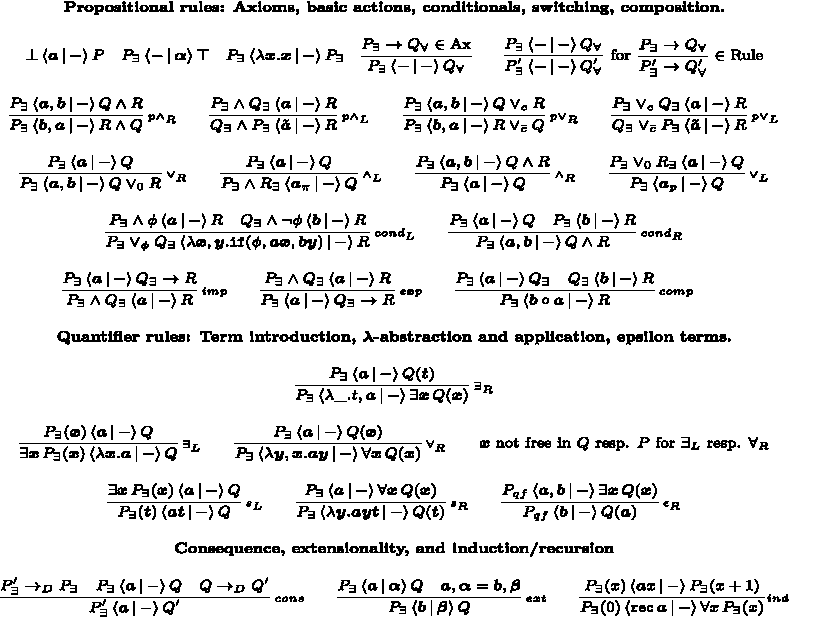
\includegraphics[width=0.95\linewidth,height=0.45\textheight,keepaspectratio]{graphic-13.pdf}\end{center}\par
 
Figure 9: Simplified rules for Dialectica triples with empty backward realiser.\par
 
% END A1.F9
 
% BEGIN A1.SS0.SSS0.P0.SPx3.p1
 
Suppose that the premises of the rule hold, and so in particular by the left hand premise\par
  
\par  \quad  \[\forall\bm{x},\bm{v}\left(|{P_{\forall}(\bm{x})}|_{\bm{\alpha}\bm{x}\bm{v}}\wedge\phi(\bm{x})\to|{P_{\forall}(\bm{a}\bm{x})}|_{\bm{v}}\right)\]\quad  \quad  
  
Writing $\bm{b}:=\mathtt{while}^{+}_{\prec}\,{\phi}\,\mathtt{do}\,{\bm{a}}$ and $\bm{\beta}:=\mathtt{while}^{-}_{\prec}\,{\phi}\,\mathtt{do}\,{(\bm{a},\bm{\alpha})}$, we are done if we can prove $\forall\bm{x}\,A(\bm{x})$ for\par
  
\par  \quad  \[A(\bm{x}):=\forall\bm{v}\left(|{P_{\forall}(\bm{x})}|_{\bm{\beta}\bm{x}\bm{v}}\to|{P_{\forall}(\bm{b}\bm{x})}|_{\bm{v}}\wedge\neg\phi(\bm{b}\bm{x})\right)\]\quad  \quad  
  
We do this using the wellfounded induction rule $\mathrm{I}_{\prec}$. So fixing $\bm{x}$, we assume that $A(\bm{y})$ holds for all $\bm{y}\prec\bm{x}$. To prove $A(\bm{x})$, we use Lemma 5, which is applicable for any $\bm{x}$ thanks to the right hand premise of $(W_{\prec})$. There are two cases to consider. If $\neg\phi(\bm{x})$ then $\bm{b}\bm{x}=\bm{x}$ and $\bm{\beta}\bm{x}=\lambda\bm{v}.\bm{v}$, and then $A(\bm{x})$ becomes\par
  
\par  \quad  \[\forall\bm{v}\left(|{P_{\forall}(\bm{x})}|_{\bm{v}}\to|{P_{\forall}(\bm{x})}|_{\bm{v}}\wedge\neg\phi(\bm{x})\right)\]\quad  \quad  
  
which is provable in this case. On the other hand, if $\phi(\bm{x})$ then we have $\bm{b}\bm{x}=\bm{b}(\bm{a}\bm{x})$, $\bm{\beta}\bm{x}=\lambda\bm{v}.\bm{\alpha}\bm{x}(\bm{\beta}(\bm{a}\bm{x})\bm{v})$ and so $A(\bm{x})$ becomes\par
  
\par  \quad  \[\forall\bm{v}\left(|{P_{\forall}(\bm{x})}|_{\bm{\alpha}\bm{x}(\bm{\beta}(\bm{a}\bm{x})\bm{v})}\to|{P_{\forall}(\bm{b}(\bm{a}\bm{x}))}|_{\bm{v}}\wedge\neg\phi(\bm{b}(\bm{a}\bm{x}))\right)\]\quad  \quad  
  
But from $\phi(\bm{x})$ we also obtain $\bm{a}\bm{x}\prec\bm{x}$, and so by the induction hypothesis we can assume\par
  
\par  \quad  \[\forall\bm{v}\left(|{P_{\forall}(\bm{a}\bm{x})}|_{\bm{\beta}(\bm{a}\bm{x})\bm{v}}\to|{P_{\forall}(\bm{b}(\bm{a}\bm{x}))}|_{\bm{v}}\wedge\neg\phi(\bm{b}(\bm{a}\bm{x}))\right)\]\quad  \quad  
  
It suffices therefore to show that\par
  
\par  \quad  \[\forall\bm{v}\left(|{P_{\forall}(\bm{x})}|_{\bm{\alpha}\bm{x}(\bm{\beta}(\bm{a}\bm{x})\bm{v})}\to|{P_{\forall}(\bm{a}\bm{x})}|_{\bm{\beta}(\bm{a}\bm{x})\bm{v}}\right)\]\quad  \quad  
  
and this is immediate from the left hand premise of $(W_{\prec})$ and the fact that $\phi(\bm{x})$ holds, and so we have completed the induction step and therefore the proof. $\hfill\blacktriangleleft$\par
 
% END A1.SS0.SSS0.P0.SPx3.p1
 
% END A1.SS0.SSS0.P0.SPx3
 
% BEGIN A1.SS0.SSS0.P0.SPx4
 
\par\medskip\noindent\textbf{Proof of Theorem 8.}\par
 
% BEGIN A1.SS0.SSS0.P0.SPx4.p1
 
For $\mathtt{skip}$ and the primitive commands this is immediate. The core of the proof lies in the composition rule. Here, for any $s$, by the induction hypothesis there exist $s^{\prime},\sigma^{\prime},\Gamma^{\prime}$ and $s^{\prime\prime},\sigma^{\prime},\Gamma^{\prime}$ such that\par
  
\par  \quad  \[\begin{cases}{s},{C_{1}}\,{\Downarrow^{+}}\,{s^{\prime}},{\sigma},{\Gamma}\\
{s^{\prime}},{C_{2}}\,{\Downarrow^{+}}\,{s^{\prime\prime}},{\sigma^{\prime}},{\Gamma^{\prime}}\end{cases}\]\quad  \quad  
  
and therefore\par
  
\par  \quad  \[{s},{{C_{1}}\,;\,{C_{2}}}\,{\Downarrow^{+}}\,{s^{\prime\prime}},{\sigma^{\prime}::\sigma},{\Gamma^{\prime}::\Gamma}\]\quad  \quad  
  
for $s^{\prime}=C_{1}^{+}s$ and $s^{\prime\prime}=C_{2}^{+}s^{\prime}=(C_{2}^{+}\circ C^{+}_{1})s=({C_{1}}\,;\,{C_{2}})^{+}s$. For the backward direction, again using the induction hypothesis, for any $t,\sigma_{0}$ and $\Gamma_{0}$ we have\par
  
\par  \quad  \[\begin{cases}{\sigma^{\prime}::\sigma::\sigma_{0}},{\Gamma^{\prime}::\Gamma::\Gamma_{0}},{t}\,{\Downarrow^{-}}\,{\sigma::\sigma_{0}},{\Gamma::\Gamma_{0}},{t^{\prime}}\\
{\sigma::\sigma_{0}},{\Gamma::\Gamma_{0}},{t^{\prime}}\,{\Downarrow^{-}}\,{\sigma_{0}},{\Gamma_{0}},{t^{\prime\prime}}\end{cases}\]\quad  \quad  
  
and therefore\par
  
\par  \quad  \[{\sigma^{\prime}::\sigma::\sigma_{0}},{\Gamma^{\prime}::\Gamma::\Gamma_{0}},{t}\,{\Downarrow^{-}}\,{\sigma_{0}},{\Gamma_{0}},{t^{\prime\prime}}\]\quad  \quad  
  
for $t^{\prime}=C_{2}^{-}s^{\prime}t$ and $t^{\prime\prime}=C_{1}^{-}st^{\prime}=C_{1}^{-}s(C_{2}^{-}s^{\prime}t)=C_{1}^{-}s(C_{2}^{-}(C_{1}^{+}s)t)=({C_{1}}\,;\,{C_{2}})^{-}st$. The conditionals are straightforward, since whenever $\phi(s)$ then in $\mathrm{WE}\mbox{-}\mathrm{HA}^{\omega}$ we have\par
  
\par  \quad  $\displaystyle(\mathtt{if}\,{\phi}\,\mathtt{then}\,{C_{1}}\,\mathtt{else}\,{C_{2}})^{+}s$\quad  $\displaystyle=C_{1}^{+}s$\quad  \quad  
 
\par  \quad  $\displaystyle(\mathtt{if}\,{\phi}\,\mathtt{then}\,{C_{1}}\,\mathtt{else}\,{C_{2}})^{-}st$\quad  $\displaystyle=C_{1}^{-}st$\quad  \quad  
  
and similarly for $\neg\phi(s)$. Finally, for the while loop we use induction on $\prec$, using that if $\phi(s)$ then $(\mathtt{while}_{\prec}\,{\phi}\,\mathtt{do}\,{C})s=({C}\,;\,{\mathtt{while}_{\prec}\,{\phi}\,\mathtt{do}\,{C}})$ (and also $(\mathtt{while}_{\prec}\,{\phi}\,\mathtt{do}\,{C})s=(\mathtt{skip})s$ if $\neg\phi(s)$), and so the induction step is essentially the same as the composition rule. $\hfill\blacktriangleleft$\par
 
% END A1.SS0.SSS0.P0.SPx4.p1
 
% BEGIN A1.SS0.SSS0.P0.SPx4.p2
 
\par
 
% END A1.SS0.SSS0.P0.SPx4.p2
 
% END A1.SS0.SSS0.P0.SPx4
 
% END A1


% BEGIN bib
 
\par\medskip\noindent\textbf{References}\par
  
\par\noindent  [1]  Wilhelm Ackermann.  Begründung des “tertium non datur” mittels der Hilbertschen Theorie der Widerspruchsfreiheit.  Mathematische Annalen, 93:1–36, 1924.  doi:10.1007/BF01449946.  
 
\par\noindent  [2]  Federico Aschieri and Stefano Berardi.  Interactive learning-based realizability for Heyting arithmetic with EM1.  Logical Methods in Computer Science, 6(3), 2010.  doi:10.2168/LMCS-6(3:19)2010.  
 
\par\noindent  [3]  Federico Aschieri, Adata Ciabattoni, and Francesco Genco.  On the concurrent computational content of intermediate logics.  Theoretical Computer Science, 813:375–409, 2020.  doi:10.1016/j.tcs.2020.01.022.  
 
\par\noindent  [4]  Jeremy Avigad, Edward T. Dean, and Jason Rute.  A metastable dominated convergence theorem.  Journal of Logic \& Analysis, 4(3):1–19, 2012.  doi:10.4115/jla.2012.4.3.  
 
\par\noindent  [5]  Jeremy Avigad, Philipp Gerhardy, and Henry Towsner.  Local stability of ergodic averages.  Transactions of the American Mathematical Society, 362(1):261–288, 2010.  doi:10.1090/S0002-9947-09-04814-4.  
 
\par\noindent  [6]  Stefano Berardi, Marc Bezem, and Thierry Coquand.  On the computational content of the axiom of choice.  Journal of Symbolic Logic, 63(2):600–622, 1998.  doi:10.2307/2586854.  
 
\par\noindent  [7]  Ulrich Berger and Helmut Schwichtenber.  Program extraction from classical proofs.  In Logic and Computational Complexity workshop (LCC’94), volume 960 of Lecture Notes in Computer Science, pages 77–97, 1995.  doi:10.1007/3-540-60178-3\_80.  
 
\par\noindent  [8]  Valeria de Paiva.  The Dialectica categories.  PhD thesis, University of Cambridge, 1991.  Published as Technical Report 213, Computer Laboratory, University of Cambridge.  doi:10.48456/tr-213.  
 
\par\noindent  [9]  Jerry den Hartog and Erik P. de Vink.  Verifying probabilistic programs using a Hoare like logic.  International Journal of Foundations of Computer Science, 13:315–340, 2002.  doi:10.1142/S012905410200114X.  
 
\par\noindent  [10]  Justus Diller.  Eine Variante zur Dialectica-Interpretation der Heyting-Arithmetik endlicher Typen.  Archiv für mathematische Logik und Grundlagenforschung, 16(1–2):49–66, 1974.  doi:10.1007/BF02025118.  
 
\par\noindent  [11]  Philipp Gerhardy and Ulrich Kohlenbach.  General logical metatheorems for functional analysis.  Transactions of the American Mathematical Society, 360:2615–2660, 2008.  doi:10.1090/S0002-9947-07-04429-7.  
 
\par\noindent  [12]  Kurt Gödel.  Über eine bisher noch nicht benützte Erweiterung des finiten Standpunktes.  dialectica, 12(3–4):280–287, 1958.  doi:10.1111/j.1746-8361.1958.tb01464.x.  
 
\par\noindent  [13]  Timothy Griffin.  A formulae-as-type notion of control.  In Proceedings of Principles of Programming Languages (POPL’90), pages 47–58. ACM, 1990.  doi:10.1145/96709.96714.  
 
\par\noindent  [14]  Charles Antony Richard Hoare.  An axiomatic basis for computer programming.  Communications of the ACM, 12(10):576–580, 1969.  doi:10.1145/363235.363259.  
 
\par\noindent  [15]  William A. Howard.  Hereditarily majorizable functionals of finite type.  In Anne S. Troelstra, editor, Metamathematical Investigation of Intuitionistic Arithmetic and Analysis, volume 344 of Lecture Notes in Mathematics. Springer-Verlag, 1973.  doi:10.1007/BFb0066739.  
 
\par\noindent  [16]  Marie Kerjean and Pierre-Marie Pédrot.  $\delta$ is for Dialectica.  In Proceedings of Logic in Computer Science (LICS’24), pages 48:1–13. ACM, 2024.  doi:10.1145/3661814.3662106.  
 
\par\noindent  [17]  Ulrich Kohlenbach.  Some logical metatheorems with applications in functional analysis.  Transactions of the American Mathematical Society, 357(1):89–128, 2005.  doi:10.1090/s0002-9947-04-03515-9.  
 
\par\noindent  [18]  Ulrich Kohlenbach.  Applied Proof Theory: Proof Interpretations and their Use in Mathematics.  Springer Monographs in Mathematics. Springer, 2008.  doi:10.1007/978-3-540-77533-1.  
 
\par\noindent  [19]  Ulrich Kohlenbach.  Recent progress in proof mining in nonlinear analysis.  IFCoLoG Journal of Logics and their Applications, 10(4):3361–3410, 2017.  URL: https://www2.mathematik.tu-darmstadt.de/˜kohlenbach/progress-new.pdf.  
 
\par\noindent  [20]  Ulrich Kohlenbach.  Proof-theoretic methods in nonlinear analysis.  In Proceedings of the International Congress of Mathematicians 2018, volume 2, pages 61–82. World Scientific, 2019.  doi:10.1142/9789813272880\_0045.  
 
\par\noindent  [21]  Ulrich Kohlenbach.  Local formalizations in nonlinear analysis and related areas and proof-theoretic tameness.  In Kreisel’s Interests: On the Foundations of Logic and Mathematics, volume 41 of Tributes, pages 45–61. College Publications, 2020.  URL: https://www2.mathematik.tu-darmstadt.de/˜kohlenbach/Kreisel2018.pdf.  
 
\par\noindent  [22]  Jean-Louis Krivine.  Realizability in classical logic. in: Interactive models of computation and program behaviour.  Panoramas et synthéses, 27:197–229, 2009.  URL: https://hal.science/hal-00154500/document.  
 
\par\noindent  [23]  Wilfried Meyer-Viol.  Instantial Logic.  PhD thesis, University of Amsterdam, 1985.  URL: https://eprints.illc.uva.nl/id/eprint/1984/2/DS-1995-11.text.pdf.  
 
\par\noindent  [24]  Alexandre Miquel.  Existential witness extraction in classical realizability and via a negative translation.  Logical Methods in Computer Science, 7(2:2):1–47, 2011.  doi:10.2168/LMCS-7(2:2)2011.  
 
\par\noindent  [25]  Morenikeji Neri and Nicholas Pischke.  Proof mining and probability theory.  Forum of Mathematics, Sigma, 13:e187, 2025.  doi:10.1017/fms.2025.10138.  
 
\par\noindent  [26]  Morenikeji Neri, Nicholas Pischke, and Thomas Powell.  Generalized learnability of stochastic principles.  In Proceedings of Computability in Europe (CiE’25), volume 15764 of LNCS, pages 333–348, 2025.  doi:10.1007/978-3-031-95908-0\_24.  
 
\par\noindent  [27]  Morenikeji Neri and Thomas Powell.  On quantitative convergence for stochastic processes: Crossings, fluctuations and martingales.  Transactions of the American Mathematical Society, Series B, 12:974–1019, 2025.  doi:10.1090/btran/229.  
 
\par\noindent  [28]  Morenikeji Neri and Thomas Powell.  A quantitative Robbins-Siegmund theorem.  Annals of Applied Probability, 2025.  To appear.  doi:10.48550/arXiv.2410.15986.  
 
\par\noindent  [29]  Peter O’Hearn and David Pym.  The logic of bunched implications.  Bulletin of Symbolic Logic, 5(2):215–244, 1999.  doi:10.2307/421090.  
 
\par\noindent  [30]  Paulo Oliva.  Unifying functional interpretations.  Notre Dame Journal of Formal Logic, 47(2):263–290, 2006.  doi:10.1305/ndjfl/1153858651.  
 
\par\noindent  [31]  Paulo Oliva.  Functional interpretations of linear and intuitionistic logic.  Information and Computation, 208(5):565–577, 2010.  doi:10.1016/j.ic.2008.11.008.  
 
\par\noindent  [32]  Michel Parigot.  $\lambda\mu$-calculus: An algorithmic interpretation of classical natural deduction.  In Proceedings of Logic Programming and Automated Reasoning (LPAR’92), pages 190–201. Springer Berlin Heidelberg, 1992.  doi:10.1007/BFb0013061.  
 
\par\noindent  [33]  Pierre-Marie Pédrot.  A functional functional interpretation.  In Joint proceedings of Computer Science Logic and Logic in Computer Science (CSL–LICS’14), pages 77:1–10. ACM, 2014.  doi:10.1145/2603088.2603094.  
 
\par\noindent  [34]  Thomas Powell.  Gödel’s functional interpretation and the concept of learning.  In Proceedings of Logic in Computer Science (LICS ’16), pages 136–145. ACM, 2016.  doi:10.1145/2933575.2933605.  
 
\par\noindent  [35]  Thomas Powell.  Computational interpretations of classical reasoning: From the epsilon calculus to stateful programs.  In Mathesis Universalis, Computability and Proof, volume 412 of Synthese Library, pages 255–290. Springer, 2019.  doi:10.1007/978-3-030-20447-1\_14.  
 
\par\noindent  [36]  Thomas Powell.  Proofs as stateful programs: A first-order logic with abstract Hoare triples.  Logical Methods in Computer Science, 20(1):7:1–7:32, 2024.  doi:10.46298/LMCS-20(1:7)2024.  
 
\par\noindent  [37]  John C. Reynolds.  Separation logic: a logic for shared mutable data structures.  In Proceedings of Logic in Computer Science (LICS’02), pages 55–74. IEEE, 2002.  doi:10.1109/LICS.2002.1029817.  
 
\par\noindent  [38]  Helmut Schwichtenberg.  Dialectica interpretation of well-founded induction.  Mathematical Logic Quarterly, 54(3):229–239, 2008.  doi:10.1002/malq.200710045.  
 
\par\noindent  [39]  Davide Trotta, Jonathan Weinberger, and Valeria de Paiva.  Skolem, Gödel, and Hilbert fibrations.  available at https://arxiv.org/abs/2407.15765, 2024.  
  
% END bib

\end{document}
